\chapter{Discrete Fourier Transform}

In mathematics, the discrete Fourier transform (DFT) converts a finite sequence of equally-spaced samples of a function into a same-length sequence of equally-spaced samples of the discrete-time Fourier transform (DTFT), which is a complex-valued function of frequency. The interval at which the DTFT is sampled is the reciprocal of the duration of the input sequence. An inverse DFT is a Fourier series, using the DTFT samples as coefficients of complex sinusoids at the corresponding DTFT frequencies. It has the same sample-values as the original input sequence. The DFT is therefore said to be a frequency domain representation of the original input sequence. If the original sequence spans all the non-zero values of a function, its DTFT is continuous (and periodic), and the DFT provides discrete samples of one cycle. If the original sequence is one cycle of a periodic function, the DFT provides all the non-zero values of one DTFT cycle.

The DFT is the most important discrete transform, used to perform Fourier analysis in many practical applications. In digital signal processing, the function is any quantity or signal that varies over time, such as the pressure of a sound wave, a radio signal, or daily temperature readings, sampled over a finite time interval (often defined by a window function). In image processing, the samples can be the values of pixels along a row or column of a raster image. The DFT is also used to efficiently solve partial differential equations, and to perform other operations such as convolutions or multiplying large integers.

Since it deals with a \textbf{finite} amount of data, it can be implemented in computers by numerical algorithms or even dedicated hardware. These implementations usually employ efficient fast Fourier transform (FFT) algorithms; so much so that the terms ``FFT'' and ``DFT'' are often used interchangeably. Prior to its current usage, the ``FFT'' initialism may have also been used for the ambiguous term ``finite Fourier transform''~\cite{bib:discreteFourierTransform}.

\section{Orthogonal Transforms}

Let $x[n]$ be a sequence of length $N$. We define $\mathcal X[k], 0 \leq k \leq N-1$ the $N$-point \textbf{orthogonal transform} of $x[n]$. An orthogonal transforms is a \emph{generalized} version of Transforms that takes the form
\begin{eqnarray}
    \mathcal X[k] = \sum_{n=0}^{N-1} x[n] \psi^*[k,n], & 0 \leq k \leq N-1, \\\label{eqn:analysisEquation}
    x[k] = \sum_{k=0}^{N-1} \mathcal X[n] \psi[k,n], & 0 \leq n \leq N-1. \label{eqn:synthesisEquation}
\end{eqnarray}
The first Equation~\ref{eqn:analysisEquation} is called \emph{Analysis equation}, while the second Equation~\ref{eqn:synthesisEquation} is said to be the \emph{Synthesis equation}. Both analysis and synthesis equations concur in the definition of the orthogonal transform. Indeed, the analysis equation allows to perform the orthogonal transformation, while implicitly the synthesis equation serves as a ``inverse'' orthogonal transform. Still, the $\psi$ are said to be \emph{basis sequences} and are of length $N$ as well as the original sequence and the orthogonal transform sequence. Basis sequences can have complex values, so generally $\psi[k, n] \in \C$. In the class of transforms to be considered in this notes of digital signal processing, all the basis sequences will satisfy the following condition,
\begin{equation}\label{eqn:orthogonalTransformsOrthogonalityCondition}
    \frac 1 N \sum_{n=0}^{N-1} \psi[k,n]\psi^*[l,n] = \left\{\begin{array}{ll}1, & l = k\\ 0, & l \neq k\end{array}\right.,
\end{equation}
a condition that substantially poses that the product \[\psi[k,n]\psi^*[l,n]\] is equal to $1$ if and only if indexes $l = k$, a property that if satisfied then the basis sequences are said to be \emph{orthogonal to each other}.

Really, in order for $\psi^*$ to be the inverse orthogonal transform, $\psi$ and $\psi^*$ have to be orthogonal to each other. This can be verified by substituting the synthesis equation~\ref{eqn:synthesisEquation} into the analysis equation~\ref{eqn:analysisEquation},
\begin{align*}
    \sum_{n=0}^{N-1} x[n] \psi^*[k,n] &= \sum_{n=0}^{N-1}\left( \frac 1 N \sum_{k=0}^{N-1} \mathcal X[k] \psi[n,k]\right)\psi^*[l,n] \\
                                      &= \sum_{k=0}^{N-1} \mathcal X[k] \left( \frac 1 N \sum_{n=0}^{N-1}\psi[n,k]\psi^*[l,n]\right) \\
                                      &= \mathcal X[l],
\end{align*}
which yields an identity. Of course, the other way around works exactly the same, hence the inverse orthogonal transform is expressed as in Equation~\ref{eqn:synthesisEquation}.

An important consequence of the orthogonality condition for orthogonal transforms is the \textbf{Energy Preservation Property}, which states that
\begin{equation}\label{eqn:energyPreservationProperty}
    \sum_{n=0}^{N-1}|x[n]|^2 = \frac 1 N \sum_{k=0}^{N-1}\left|\mathcal X[n]\right|^2
\end{equation}
Yet, the Energy Preservation Property is more commonly known as the \emph{Parseval's Theorem}, of which it is a more general formulation.

\section{Definition of Discrete Fourier Transform}

It's now the time to introduce the \textbf{Discrete Fourier Transform (DFT)}, a tool of a paramount importance in the field of digital signal processing.

\begin{defin}[Discrete Fourier Transform]
    Let $x[n]$ be a finite-length sequence of length $N$ defined for $0 \leq n \leq N-1$ and be $X(e^{j\omega})$ its discrete-time Fourier Transform as in Equation~\ref{eqn:discreteTimeFourierTransform}. By \emph{uniformly sampling} $X(e^{j\omega})$ on the $\omega$ axis in the interval $[0, 2\pi[$ at samples $\omega_k=\frac{2k\pi}{N}$ for $0 \leq k \leq N-1$ one obtains a sequence $X[k]$ such that
    \begin{equation}\label{eqn:discreteFourierTransform}
        X[k] = X(e^{j\omega})\Bigr\rvert_{\omega = \frac {2k\pi}{N}} = \sum_{n=0}^{N-1} x[n] e^{-2j\pi \frac{k n}{N}}, 0 \leq k \leq N-1
    \end{equation}
    where $X[k]$ is a sequence of length $N$ in the frequency domain represented by the variable $k$. The sequence $X[k]$ is called the \emph{Discrete Fourier Transform (DFT)} of the sequence.
\end{defin}

The above definition has been obtained by sampling the $\omega$ frequency variable in samples $2k\pi / N$ so that the complex continuous exponential $e^{-j\omega}$ has become $e^{-2j\pi \frac{kn}{N}}$. Usually, in order to streamline the notation, the substitution
\begin{equation}\label{eqn:dftNotationWn}
    W_N = e^{-j\frac{2\pi}{N}}
\end{equation}
under which the Discrete Fourier Transform now is rewritten into the following,
\begin{equation}\label{eqn:discreteTimeFourierTransformWn}
        X[k] = \sum_{n=0}^{N-1} x[n] W_N^{kn}, 0 \leq k \leq N-1.
\end{equation}

The notation expressed in~\ref{eqn:dftNotationWn} renders the orthogonal transform operator $W_N$ in Discrete Fourier Transform sum have a positive sign in its exponents. This behavior is the opposite of what one encounters by looking at the original definition.

Along with the DFT, the \textbf{Inverse Discrete Fourier Transform} should be defined as well in order to produce meaningful computations. Indeed,
\begin{equation}\label{eqn:inverseDiscreteFourierTransformWn}
    x[k] = \sum_{k=0}^{N-1} X[k] W_N^{-kn}, 0 \leq n \leq N-1,
\end{equation}
expressed under the new notation\footnote{
    The original Discrete Fourier Transform---without employing the new notation---would be
    \[
        x[k] = \sum_{k=0}^{N-1} X[k] e^{2j\pi\frac{kn}{N}}, 0 \leq n \leq N-1,
    \]
    showing a positive sign at the exponentiation.
}.
Verifying the above inverse transform is straightforward, as it is enough to substitute the original transform into the inverse, then multiply both sides of the equation by $W_N^{ln}$ and sum the result from $n=0$ to $n=N-1$. Of course,
\begin{align*}
    \sum_{n=0}^{N-1} x[n] W_N^{ln}
    &= \sum_{n=0}^{N-1}\left(\frac 1 N\sum_{k=0}^{K-1} X[k] W_N^{-kn}\right)W_n^{ln}\\
    &= \frac 1 N \sum_{n=0}^{N-1}\sum_{k=0}^{K-1} X[k] W_N^{-(k-l)n}\\
    &= \frac 1 N \sum_{k=0}^{K-1} X[k] \left(\sum_{n=0}^{N-1}W_N^{-(k-l)n}\right).
\end{align*}
Now, since
\begin{equation}\label{eqn:dftWnProperty}
    \sum_{n=0}^{N-1}W_N^{-(k-l)n} = \left\{\begin{array}{ll} N, & k - l = rN, r \in \Z\\ 0, & \mbox{otherwise}\end{array}\right.
\end{equation}
due to the exponentiation properties. In order to verify that, just substitute with the definition of $W_N$, that is \[\sum_{n=0}^{N-1}e^{+2j\pi\frac{(k-l)n}{N}},\] a quantity that indeed is equal to $N$ if and only if $k-l$ is a multiple of $N$ and $0$ otherwise. The term relative to $n=0$ is the sum of $N$ terms all equal to $1$, while the term for $n\neq 0$ is related to the first $N$ terms of a geometric progression, that are \[\sum_{n=0}^{N-1}\rho^n = \frac{1-\rho^N}{1 - \rho} = 0\] as the exponential $e^{j2\pi\frac{N}{N}} = 1$. Another way to see it is to consider that a set of $W_N$ vectors is summed together---when $k\neq l$ for each vector of phase $\varphi$ another vector of opposite phase $-\varphi$ is summed, and the result of the sum is exactly $0$; on contrary, the only way to avoid the cancellation of terms is when $k = l$, that is when all terms have magnitude equal to $|e^{j2\pi\frac{N}{N}}| = 1$ and possess phase $\varphi = 0$. For this reason, one obtains that the only non-zero term in the sum is $\sum_{n=0}^{N-1} W_N^{-(k-l)n}, k=l, 0\leq l,k \leq N-1$. Hence,
\begin{align*}
    \sum_{n=0}^{N-1} x[n] W_N^{ln}
    &= \frac 1 N \sum_{k=0}^{K-1} X[k] \left(\sum_{n=0}^{N-1}W_N^{-(k-l)n}\right).\\
    &= \frac 1 N X[l] N = X[l].
\end{align*}

The first example in exam is a DFT of the following sequence of length $N$,
\[
    x[n] = \left\{\begin{array}{ll}
            1 & n=0\\
            0 & 1 \leq n \leq N-1
        \end{array}\right.
\]
that is quite similar to the delta impulse. Its $N$-point Discrete Fourier Transform is given by
\[
    X[k] = \sum_{n=0}^{N-1} x[n]W_N^{kn} = x[0]W_N^{k0} = 1, 1\leq k \leq N-1.
\]

The second example is of a sequence
\[
    y[n] = \left\{\begin{array}{ll}
            1 & n=m\\
            0 & 0\leq n \leq m-1, m+1 \leq n \leq N-1
        \end{array}\right.
\]
which is like the previous example, but translated of $m$. Its Discrete Fourier Transform will be
\[
    Y[k] = \sum_{n=0}^{N-1} y[n]W_N^{kn} = y[m]W_N^{km} = W_N^{km}, 1\leq k \leq N-1.
\]

Let now $g[n] = \cos{2\pi \frac{rn}{N}}$ be a sequence of length $N$. Since
\begin{align*}
    g[n] &= \frac 1 2 \left(e^{j2\pi \frac{rn}{N}} + e^{-j2\pi \frac{rn}{N}}\right)\\
         &= \frac 1 2 \left(W_N^{rn} + W_N^{rn}\right),
\end{align*}
and due to linearity the Discrete Fourier Transform will be the transform of the two addends. Therefore,
\begin{align*}
    G[k] &= \sum_{n=0}^{N-1} g[n] W_N^{kn} \\
         &= \frac 1 2 \left(\sum_{n=0}^{N-1} W_N^{-(r-k)n} + \sum_{n=0}^{N-1} W_N^{-(r+k)n}\right)
\end{align*}
and by means of Identity~\ref{eqn:dftWnProperty} one finally obtains that
\[
    G[k] = \left\{\begin{array}{ll}
            \frac N 2 & k = r\\
            \frac N 2 & k = N - r\\
            0         & \mbox{ otherwise }
    \end{array}\right.
\]

The DFT of a cosine wave is a pair of impulses of amplitude $\frac N 2$, located at samples $r$ and $N-r$ that represent \emph{the same} frequency. Conceptually then, a cosine DFT is a pair of impulses just like in the case of the Discrete-time Fourier Transform.

\subsection{Matrix relations}

Discrete Fourier Transform as expressed in~\ref{eqn:discreteTimeFourierTransformWn} can be easily expressed into a matrix form. Let $\bm x$ and $\bm X$ be two column vectors as defined,
\[
    \bm{x} = \begin{bmatrix} x[0] \\ x[1] \\ \vdots \\ x[N-1] \end{bmatrix}
    \bm{X} = \begin{bmatrix} X[0] \\ X[1] \\ \vdots \\ X[N-1] \end{bmatrix}
\]
the \emph{Matrix form of the Discrete Fourier Transform} is
\begin{equation}\label{eqn:dftMatrixForm}
    \bm{X} = \bm{D}_N\bm{x}
\end{equation}
with $\bm D_N$ the \textbf{DFT Matrix}, a $N \times N$ matrix given by
\begin{equation}\label{eqn:dftMatrixDn}
    \bm D_N = \begin{bmatrix}
        1 & 1 & 1 & \cdots & 1 \\
        1 & W_N^1 & W_N^2 & \cdots & W_N^{(N-1)} \\
        1 & W_N^2 & W_N^4 & \cdots & W_N^{2(N-1)} \\
        \vdots & \vdots & \vdots & \ddots & \vdots \\
        1 & W_N^{(N-1)} & W_N^{2(N-1)} & \cdots & W_N^{(N-1)^2} \\
    \end{bmatrix}
\end{equation}

Conversely, the \emph{Matrix form of the Inverse Discrete Fourier Transform} is given by a similar relationship,
\begin{equation}\label{eqn:idftMatrixForm}
    \bm{x} = \bm{D}^{-1}_N\bm{X}
\end{equation}
with $\bm D_N$ the \textbf{Inverse DFT Matrix}, a $N \times N$ matrix given by
\begin{equation}\label{eqn:idftMatrixDn}
    \bm D^{-1}_N = \frac 1 N\begin{bmatrix}
        1 & 1 & 1 & \cdots & 1 \\
        1 & W_N^{-1} & W_N^{-2} & \cdots & W_N^{-(N-1)} \\
        1 & W_N^{-2} & W_N^{-4} & \cdots & W_N^{-2(N-1)} \\
        \vdots & \vdots & \vdots & \ddots & \vdots \\
        1 & W_N^{-(N-1)} & W_N^{-2(N-1)} & \cdots & W_N^{-(N-1)^2} \\
    \end{bmatrix}
\end{equation}

Remarkably, the following relationship holds between the inverse and the straight DFT Matrix,
\[
    \bm D_N = \frac 1 N \bm D^{-1}_N,
\]
with a factor of $\frac 1 N$ between the one and the other.

Matrix relations are crucial to learn how to manipulate Discrete Fourier Transforms in \textsc{Matlab}. In fact, the two functions \texttt{fft} and \texttt{ifft}---which stand for \emph{Fast Fourier Transform} and \emph{Inverse Fast Fourier Transform}---manipulate column vector data structures. These two functions make use of sophisticated techniques and efficient algorithms based on the ``dividi et impera'' concept to optimize the computation of the DFT.

Let's study the DFT of the cosine $\cos{2\pi r \frac{n}{N}}$. The following \texttt{octave} code computes and plots the DFT of such function, first by setting $r=3$, then with $r=3.3$.
\begin{verbatim}
N = 21;
M = 21;
r = 3; n = 0:N-1;  u = cos(2*pi*r*n/N);
U = fft(u,M);
figure(1);
subplot(2,3,1);   n = 0:1:N-1;   stem(n,u);
title('Original time-domain sequence');
xlabel('Time index n'); ylabel('Amplitude')
subplot(2,3,2);   k = 0:1:M-1;   stem(k,abs(U));
title('Magnitude, r = 3');
xlabel('Frequency index k'); ylabel('Magnitude')
subplot(2,3,3);   stem(k,angle(U));
title('Phase, r = 3');
xlabel('Frequency index k'); ylabel('Phase')
\end{verbatim}

\begin{verbatim}
r = 3.3; n = 0:N-1;  u = cos(2*pi*r*n/N);
U = fft(u,M);
subplot(2,3,4);   n = 0:1:N-1;   stem(n,u);
title('Original time-domain sequence');
xlabel('Time index n'); ylabel('Amplitude')
subplot(2,3,5);   k = 0:1:M-1;   stem(k,abs(U));
title('Magnitude, r = 3.3');
xlabel('Frequency index k'); ylabel('Magnitude')
subplot(2,3,6);   stem(k,angle(U));
title('Phase, r = 3.3');
xlabel('Frequency index k'); ylabel('Phase')
\end{verbatim}

\begin{figure*}[ht]
\begin{center}
\scalebox{0.6}{
% Title: gl2ps_renderer figure
% Creator: GL2PS 1.4.2, (C) 1999-2020 C. Geuzaine
% For: Octave
% CreationDate: Wed Oct 19 16:31:04 2022
\setlength{\unitlength}{1pt}
\begin{picture}(0,0)
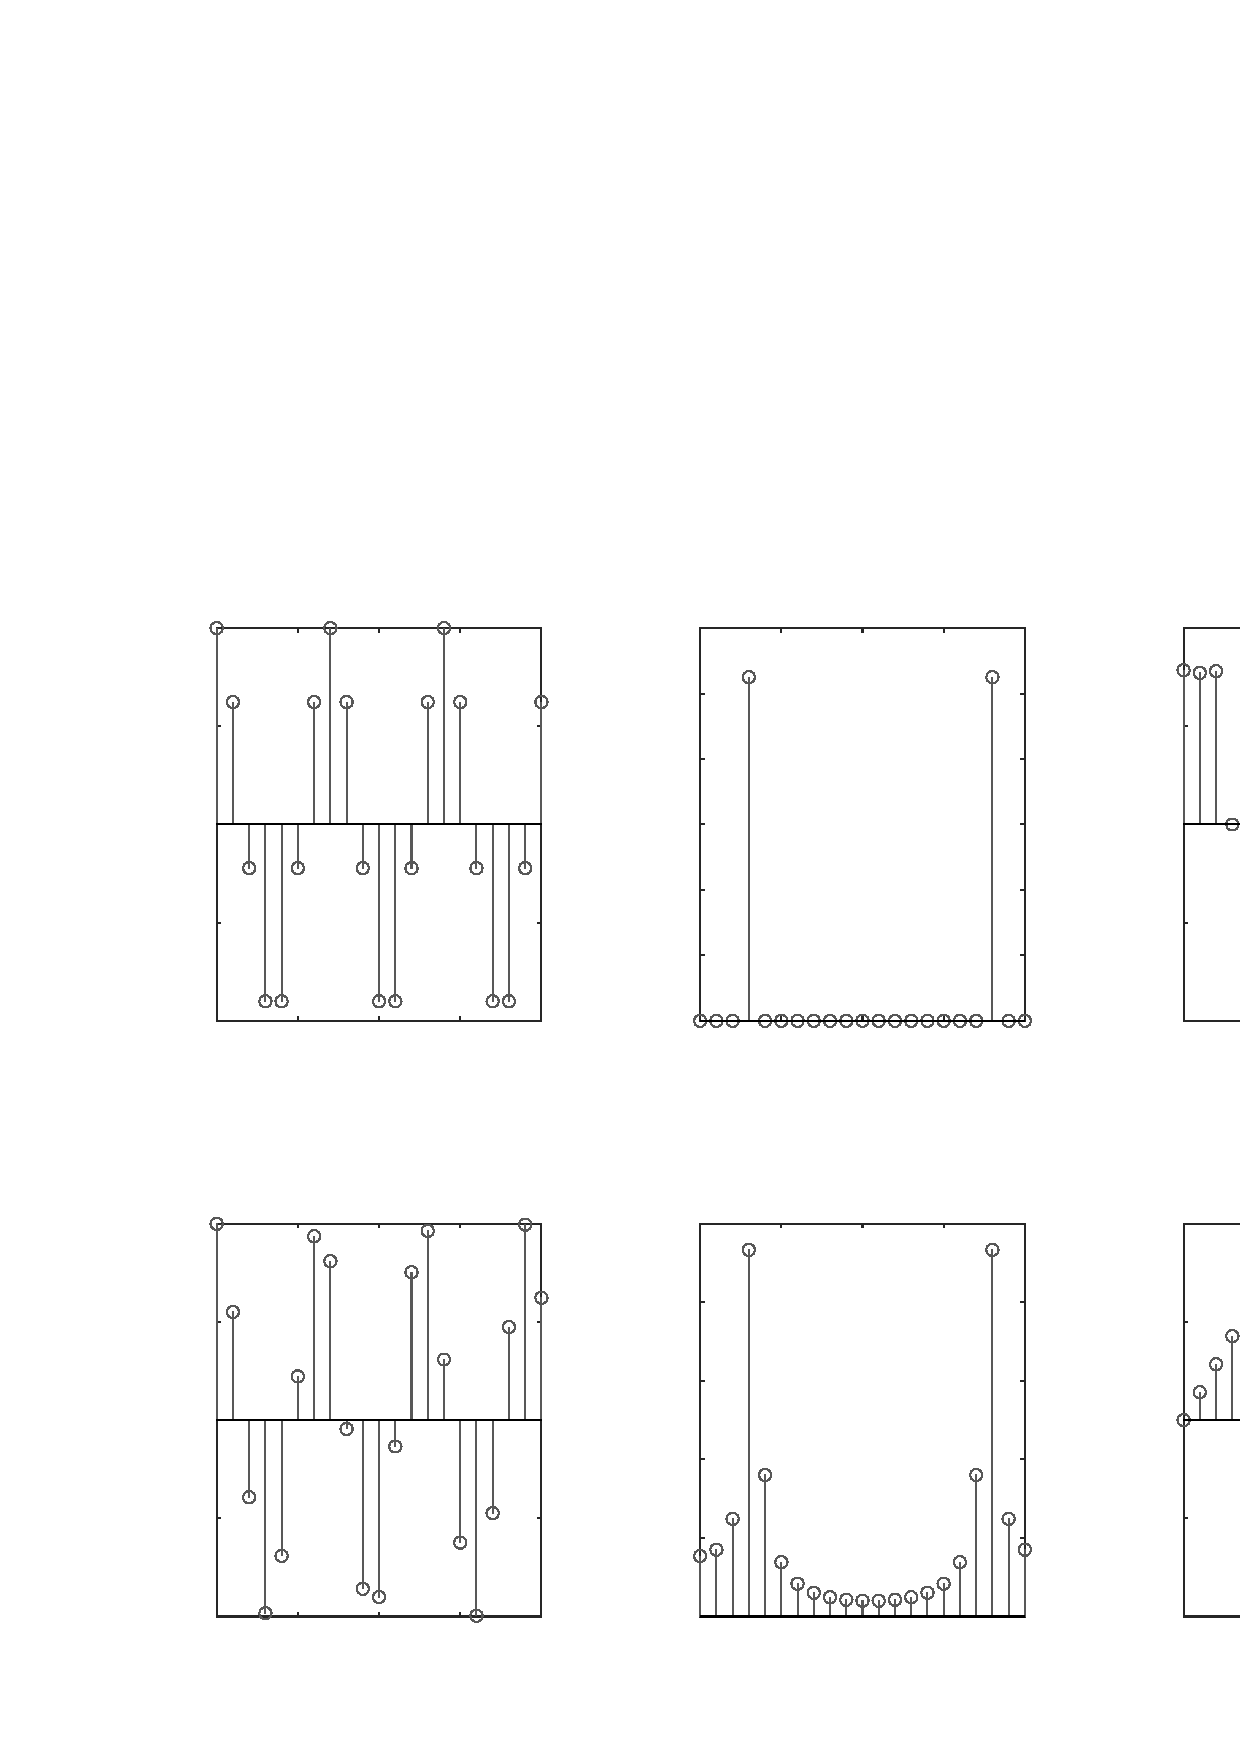
\includegraphics[scale=1]{octaves/dftCosine-inc}
\end{picture}%
\begin{picture}(800,600)(0,0)
\fontsize{13}{0}\selectfont\put(104,341.53){\makebox(0,0)[t]{\textcolor[rgb]{0.15,0.15,0.15}{{0}}}}
\fontsize{13}{0}\selectfont\put(142.97,341.53){\makebox(0,0)[t]{\textcolor[rgb]{0.15,0.15,0.15}{{5}}}}
\fontsize{13}{0}\selectfont\put(181.94,341.53){\makebox(0,0)[t]{\textcolor[rgb]{0.15,0.15,0.15}{{10}}}}
\fontsize{13}{0}\selectfont\put(220.91,341.53){\makebox(0,0)[t]{\textcolor[rgb]{0.15,0.15,0.15}{{15}}}}
\fontsize{13}{0}\selectfont\put(259.88,341.53){\makebox(0,0)[t]{\textcolor[rgb]{0.15,0.15,0.15}{{20}}}}
\fontsize{13}{0}\selectfont\put(97.0579,351.924){\makebox(0,0)[r]{\textcolor[rgb]{0.15,0.15,0.15}{{-1}}}}
\fontsize{13}{0}\selectfont\put(97.0579,399.049){\makebox(0,0)[r]{\textcolor[rgb]{0.15,0.15,0.15}{{-0.5}}}}
\fontsize{13}{0}\selectfont\put(97.0579,446.174){\makebox(0,0)[r]{\textcolor[rgb]{0.15,0.15,0.15}{{0}}}}
\fontsize{13}{0}\selectfont\put(97.0579,493.299){\makebox(0,0)[r]{\textcolor[rgb]{0.15,0.15,0.15}{{0.5}}}}
\fontsize{13}{0}\selectfont\put(97.0579,540.424){\makebox(0,0)[r]{\textcolor[rgb]{0.15,0.15,0.15}{{1}}}}
\fontsize{15}{0}\selectfont\put(181.94,550.424){\makebox(0,0)[b]{\textcolor[rgb]{0,0,0}{{Original time-domain sequence}}}}
\fontsize{15}{0}\selectfont\put(68.0579,446.174){\rotatebox{90}{\makebox(0,0)[b]{\textcolor[rgb]{0.15,0.15,0.15}{{Amplitude}}}}}
\fontsize{15}{0}\selectfont\put(181.94,325.53){\makebox(0,0)[t]{\textcolor[rgb]{0.15,0.15,0.15}{{Time index n}}}}
\fontsize{13}{0}\selectfont\put(336.06,341.53){\makebox(0,0)[t]{\textcolor[rgb]{0.15,0.15,0.15}{{0}}}}
\fontsize{13}{0}\selectfont\put(375.03,341.53){\makebox(0,0)[t]{\textcolor[rgb]{0.15,0.15,0.15}{{5}}}}
\fontsize{13}{0}\selectfont\put(414,341.53){\makebox(0,0)[t]{\textcolor[rgb]{0.15,0.15,0.15}{{10}}}}
\fontsize{13}{0}\selectfont\put(452.97,341.53){\makebox(0,0)[t]{\textcolor[rgb]{0.15,0.15,0.15}{{15}}}}
\fontsize{13}{0}\selectfont\put(491.94,341.53){\makebox(0,0)[t]{\textcolor[rgb]{0.15,0.15,0.15}{{20}}}}
\fontsize{13}{0}\selectfont\put(329.118,351.924){\makebox(0,0)[r]{\textcolor[rgb]{0.15,0.15,0.15}{{0}}}}
\fontsize{13}{0}\selectfont\put(329.118,383.34){\makebox(0,0)[r]{\textcolor[rgb]{0.15,0.15,0.15}{{2}}}}
\fontsize{13}{0}\selectfont\put(329.118,414.757){\makebox(0,0)[r]{\textcolor[rgb]{0.15,0.15,0.15}{{4}}}}
\fontsize{13}{0}\selectfont\put(329.118,446.174){\makebox(0,0)[r]{\textcolor[rgb]{0.15,0.15,0.15}{{6}}}}
\fontsize{13}{0}\selectfont\put(329.118,477.59){\makebox(0,0)[r]{\textcolor[rgb]{0.15,0.15,0.15}{{8}}}}
\fontsize{13}{0}\selectfont\put(329.118,509.007){\makebox(0,0)[r]{\textcolor[rgb]{0.15,0.15,0.15}{{10}}}}
\fontsize{13}{0}\selectfont\put(329.118,540.424){\makebox(0,0)[r]{\textcolor[rgb]{0.15,0.15,0.15}{{12}}}}
\fontsize{15}{0}\selectfont\put(414,550.424){\makebox(0,0)[b]{\textcolor[rgb]{0,0,0}{{Magnitude, r = 3}}}}
\fontsize{15}{0}\selectfont\put(308.118,446.174){\rotatebox{90}{\makebox(0,0)[b]{\textcolor[rgb]{0.15,0.15,0.15}{{Magnitude}}}}}
\fontsize{15}{0}\selectfont\put(414,325.53){\makebox(0,0)[t]{\textcolor[rgb]{0.15,0.15,0.15}{{Frequency index k}}}}
\fontsize{13}{0}\selectfont\put(568.12,341.53){\makebox(0,0)[t]{\textcolor[rgb]{0.15,0.15,0.15}{{0}}}}
\fontsize{13}{0}\selectfont\put(607.09,341.53){\makebox(0,0)[t]{\textcolor[rgb]{0.15,0.15,0.15}{{5}}}}
\fontsize{13}{0}\selectfont\put(646.06,341.53){\makebox(0,0)[t]{\textcolor[rgb]{0.15,0.15,0.15}{{10}}}}
\fontsize{13}{0}\selectfont\put(685.03,341.53){\makebox(0,0)[t]{\textcolor[rgb]{0.15,0.15,0.15}{{15}}}}
\fontsize{13}{0}\selectfont\put(724,341.53){\makebox(0,0)[t]{\textcolor[rgb]{0.15,0.15,0.15}{{20}}}}
\fontsize{13}{0}\selectfont\put(561.178,351.924){\makebox(0,0)[r]{\textcolor[rgb]{0.15,0.15,0.15}{{-4}}}}
\fontsize{13}{0}\selectfont\put(561.178,399.049){\makebox(0,0)[r]{\textcolor[rgb]{0.15,0.15,0.15}{{-2}}}}
\fontsize{13}{0}\selectfont\put(561.178,446.174){\makebox(0,0)[r]{\textcolor[rgb]{0.15,0.15,0.15}{{0}}}}
\fontsize{13}{0}\selectfont\put(561.178,493.299){\makebox(0,0)[r]{\textcolor[rgb]{0.15,0.15,0.15}{{2}}}}
\fontsize{13}{0}\selectfont\put(561.178,540.424){\makebox(0,0)[r]{\textcolor[rgb]{0.15,0.15,0.15}{{4}}}}
\fontsize{15}{0}\selectfont\put(646.06,550.424){\makebox(0,0)[b]{\textcolor[rgb]{0,0,0}{{Phase, r = 3}}}}
\fontsize{15}{0}\selectfont\put(543.178,446.174){\rotatebox{90}{\makebox(0,0)[b]{\textcolor[rgb]{0.15,0.15,0.15}{{Phase}}}}}
\fontsize{15}{0}\selectfont\put(646.06,325.53){\makebox(0,0)[t]{\textcolor[rgb]{0.15,0.15,0.15}{{Frequency index k}}}}
\fontsize{13}{0}\selectfont\put(104,55.6063){\makebox(0,0)[t]{\textcolor[rgb]{0.15,0.15,0.15}{{0}}}}
\fontsize{13}{0}\selectfont\put(142.97,55.6063){\makebox(0,0)[t]{\textcolor[rgb]{0.15,0.15,0.15}{{5}}}}
\fontsize{13}{0}\selectfont\put(181.94,55.6063){\makebox(0,0)[t]{\textcolor[rgb]{0.15,0.15,0.15}{{10}}}}
\fontsize{13}{0}\selectfont\put(220.91,55.6063){\makebox(0,0)[t]{\textcolor[rgb]{0.15,0.15,0.15}{{15}}}}
\fontsize{13}{0}\selectfont\put(259.88,55.6063){\makebox(0,0)[t]{\textcolor[rgb]{0.15,0.15,0.15}{{20}}}}
\fontsize{13}{0}\selectfont\put(97.0579,66){\makebox(0,0)[r]{\textcolor[rgb]{0.15,0.15,0.15}{{-1}}}}
\fontsize{13}{0}\selectfont\put(97.0579,113.125){\makebox(0,0)[r]{\textcolor[rgb]{0.15,0.15,0.15}{{-0.5}}}}
\fontsize{13}{0}\selectfont\put(97.0579,160.25){\makebox(0,0)[r]{\textcolor[rgb]{0.15,0.15,0.15}{{0}}}}
\fontsize{13}{0}\selectfont\put(97.0579,207.375){\makebox(0,0)[r]{\textcolor[rgb]{0.15,0.15,0.15}{{0.5}}}}
\fontsize{13}{0}\selectfont\put(97.0579,254.5){\makebox(0,0)[r]{\textcolor[rgb]{0.15,0.15,0.15}{{1}}}}
\fontsize{15}{0}\selectfont\put(181.94,264.5){\makebox(0,0)[b]{\textcolor[rgb]{0,0,0}{{Original time-domain sequence}}}}
\fontsize{15}{0}\selectfont\put(68.0579,160.25){\rotatebox{90}{\makebox(0,0)[b]{\textcolor[rgb]{0.15,0.15,0.15}{{Amplitude}}}}}
\fontsize{15}{0}\selectfont\put(181.94,39.6063){\makebox(0,0)[t]{\textcolor[rgb]{0.15,0.15,0.15}{{Time index n}}}}
\fontsize{13}{0}\selectfont\put(336.06,55.6063){\makebox(0,0)[t]{\textcolor[rgb]{0.15,0.15,0.15}{{0}}}}
\fontsize{13}{0}\selectfont\put(375.03,55.6063){\makebox(0,0)[t]{\textcolor[rgb]{0.15,0.15,0.15}{{5}}}}
\fontsize{13}{0}\selectfont\put(414,55.6063){\makebox(0,0)[t]{\textcolor[rgb]{0.15,0.15,0.15}{{10}}}}
\fontsize{13}{0}\selectfont\put(452.97,55.6063){\makebox(0,0)[t]{\textcolor[rgb]{0.15,0.15,0.15}{{15}}}}
\fontsize{13}{0}\selectfont\put(491.94,55.6063){\makebox(0,0)[t]{\textcolor[rgb]{0.15,0.15,0.15}{{20}}}}
\fontsize{13}{0}\selectfont\put(329.118,66){\makebox(0,0)[r]{\textcolor[rgb]{0.15,0.15,0.15}{{0}}}}
\fontsize{13}{0}\selectfont\put(329.118,103.7){\makebox(0,0)[r]{\textcolor[rgb]{0.15,0.15,0.15}{{2}}}}
\fontsize{13}{0}\selectfont\put(329.118,141.4){\makebox(0,0)[r]{\textcolor[rgb]{0.15,0.15,0.15}{{4}}}}
\fontsize{13}{0}\selectfont\put(329.118,179.1){\makebox(0,0)[r]{\textcolor[rgb]{0.15,0.15,0.15}{{6}}}}
\fontsize{13}{0}\selectfont\put(329.118,216.8){\makebox(0,0)[r]{\textcolor[rgb]{0.15,0.15,0.15}{{8}}}}
\fontsize{13}{0}\selectfont\put(329.118,254.5){\makebox(0,0)[r]{\textcolor[rgb]{0.15,0.15,0.15}{{10}}}}
\fontsize{15}{0}\selectfont\put(414,264.5){\makebox(0,0)[b]{\textcolor[rgb]{0,0,0}{{Magnitude, r = 3.3}}}}
\fontsize{15}{0}\selectfont\put(308.118,160.25){\rotatebox{90}{\makebox(0,0)[b]{\textcolor[rgb]{0.15,0.15,0.15}{{Magnitude}}}}}
\fontsize{15}{0}\selectfont\put(414,39.6063){\makebox(0,0)[t]{\textcolor[rgb]{0.15,0.15,0.15}{{Frequency index k}}}}
\fontsize{13}{0}\selectfont\put(568.12,55.6063){\makebox(0,0)[t]{\textcolor[rgb]{0.15,0.15,0.15}{{0}}}}
\fontsize{13}{0}\selectfont\put(607.09,55.6063){\makebox(0,0)[t]{\textcolor[rgb]{0.15,0.15,0.15}{{5}}}}
\fontsize{13}{0}\selectfont\put(646.06,55.6063){\makebox(0,0)[t]{\textcolor[rgb]{0.15,0.15,0.15}{{10}}}}
\fontsize{13}{0}\selectfont\put(685.03,55.6063){\makebox(0,0)[t]{\textcolor[rgb]{0.15,0.15,0.15}{{15}}}}
\fontsize{13}{0}\selectfont\put(724,55.6063){\makebox(0,0)[t]{\textcolor[rgb]{0.15,0.15,0.15}{{20}}}}
\fontsize{13}{0}\selectfont\put(561.178,66){\makebox(0,0)[r]{\textcolor[rgb]{0.15,0.15,0.15}{{-2}}}}
\fontsize{13}{0}\selectfont\put(561.178,113.125){\makebox(0,0)[r]{\textcolor[rgb]{0.15,0.15,0.15}{{-1}}}}
\fontsize{13}{0}\selectfont\put(561.178,160.25){\makebox(0,0)[r]{\textcolor[rgb]{0.15,0.15,0.15}{{0}}}}
\fontsize{13}{0}\selectfont\put(561.178,207.375){\makebox(0,0)[r]{\textcolor[rgb]{0.15,0.15,0.15}{{1}}}}
\fontsize{13}{0}\selectfont\put(561.178,254.5){\makebox(0,0)[r]{\textcolor[rgb]{0.15,0.15,0.15}{{2}}}}
\fontsize{15}{0}\selectfont\put(646.06,264.5){\makebox(0,0)[b]{\textcolor[rgb]{0,0,0}{{Phase, r = 3.3}}}}
\fontsize{15}{0}\selectfont\put(543.178,160.25){\rotatebox{90}{\makebox(0,0)[b]{\textcolor[rgb]{0.15,0.15,0.15}{{Phase}}}}}
\fontsize{15}{0}\selectfont\put(646.06,39.6063){\makebox(0,0)[t]{\textcolor[rgb]{0.15,0.15,0.15}{{Frequency index k}}}}
\end{picture}

}\caption{Plots of original signal (left), magnitude (center) and phase (right) of the Discrete Fourier Transform of sequence $\cos{2\pi r \frac{n}{N}}$. Notice how two perfect impulses are generated if and only if the quantity $r$ is an integer.}\label{oct:dftCosine}
\end{center}
\end{figure*}

The Discrete Fourier Transform of a cosine wave will produce a peculiar \emph{pair of impulses} located at the very same frequency of the sinusoid, provided the multiplying factor of $n$ is a \emph{multiple of $2\pi$}---that is, when $r \in \Z$. In all other cases, imperfect impulses will be generated, a phenomenon that is quite visible in Figure~\ref{oct:dftCosine} for the case of $r=3.3$.

The DFT of the delta impulse can be produced by running the following \texttt{octave} code, that will first generate three pictures like those in Figure~\ref{oct:dftCosine} related to a $\delta[n]$ sequence, then it will do the same with a delayed delta impulse,
\begin{verbatim}
N = 21;
M = 21;
u = [1 zeros(1,N-1)];
U = fft(u,M);
figure(1);
subplot(2,3,1);   n = 0:1:N-1;   stem(n,u);
title('Impulse in zero');
xlabel('Time index n'); ylabel('Amplitude')
subplot(2,3,2);   k = 0:1:M-1;   stem(k,abs(U));
title('Magnitude');
xlabel('Frequency index k'); ylabel('Magnitude')
subplot(2,3,3);   stem(k,angle(U));
title('Phase');
xlabel('Frequency index k'); ylabel('Phase')
\end{verbatim}

\begin{verbatim}
u = [zeros(1,4) 1 zeros(1,N-5)];
U = fft(u,M);
subplot(2,3,4);   n = 0:1:N-1;   stem(n,u);
title('Delayed impulse');
xlabel('Time index n'); ylabel('Amplitude')
subplot(2,3,5);   k = 0:1:M-1;   stem(k,abs(U));
title('Magnitude');
xlabel('Frequency index k'); ylabel('Magnitude')
subplot(2,3,6);   stem(k,angle(U));
title('Phase');
xlabel('Frequency index k'); ylabel('Phase')
\end{verbatim}



\begin{figure*}[ht]
\begin{center}
\scalebox{0.6}{
% Title: gl2ps_renderer figure
% Creator: GL2PS 1.4.2, (C) 1999-2020 C. Geuzaine
% For: Octave
% CreationDate: Wed Oct 19 16:35:19 2022
\setlength{\unitlength}{1pt}
\begin{picture}(0,0)
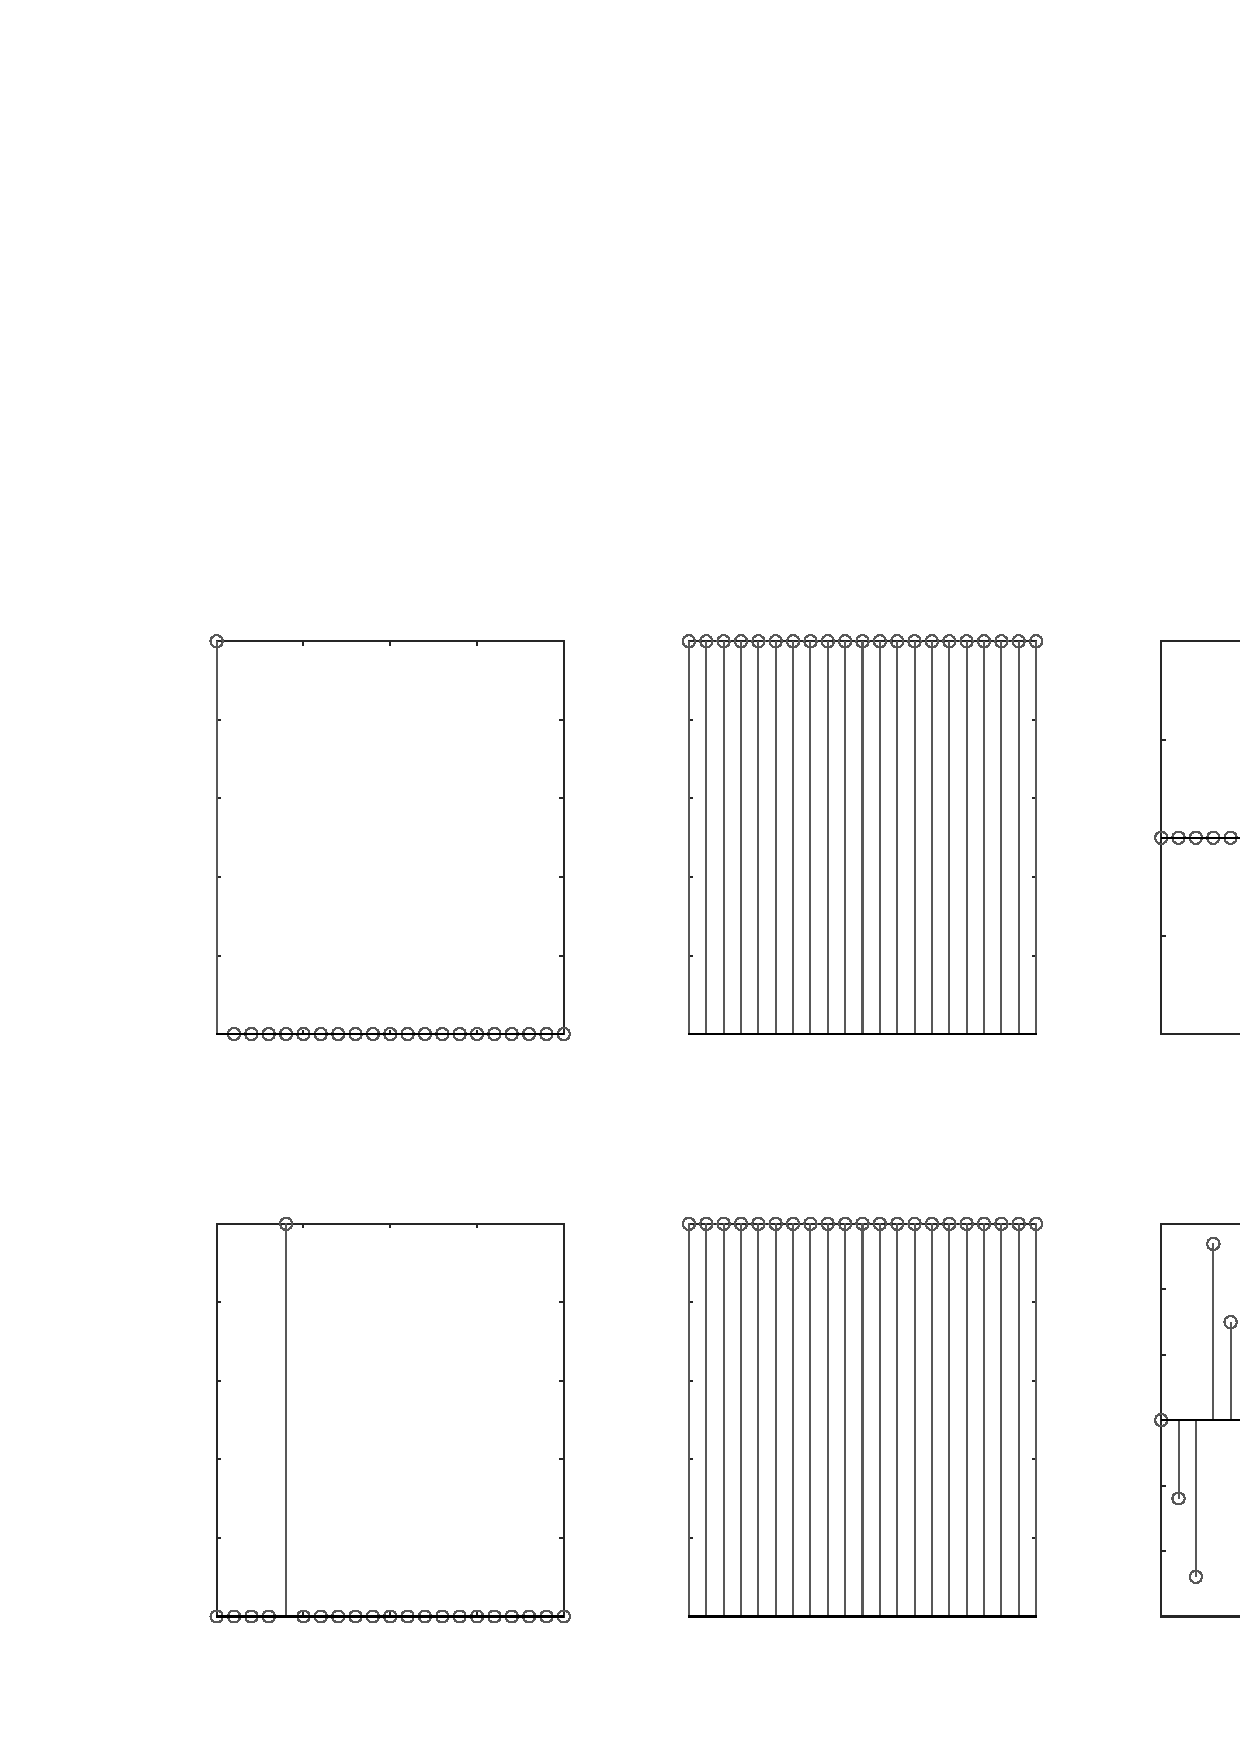
\includegraphics[scale=1]{octaves/dftImpulse-inc}
\end{picture}%
\begin{picture}(800,600)(0,0)
\fontsize{13}{0}\selectfont\put(104,335.173){\makebox(0,0)[t]{\textcolor[rgb]{0.15,0.15,0.15}{{0}}}}
\fontsize{13}{0}\selectfont\put(145.658,335.173){\makebox(0,0)[t]{\textcolor[rgb]{0.15,0.15,0.15}{{5}}}}
\fontsize{13}{0}\selectfont\put(187.316,335.173){\makebox(0,0)[t]{\textcolor[rgb]{0.15,0.15,0.15}{{10}}}}
\fontsize{13}{0}\selectfont\put(228.973,335.173){\makebox(0,0)[t]{\textcolor[rgb]{0.15,0.15,0.15}{{15}}}}
\fontsize{13}{0}\selectfont\put(270.631,335.173){\makebox(0,0)[t]{\textcolor[rgb]{0.15,0.15,0.15}{{20}}}}
\fontsize{13}{0}\selectfont\put(97.0679,345.566){\makebox(0,0)[r]{\textcolor[rgb]{0.15,0.15,0.15}{{0}}}}
\fontsize{13}{0}\selectfont\put(97.0679,383.266){\makebox(0,0)[r]{\textcolor[rgb]{0.15,0.15,0.15}{{0.2}}}}
\fontsize{13}{0}\selectfont\put(97.0679,420.966){\makebox(0,0)[r]{\textcolor[rgb]{0.15,0.15,0.15}{{0.4}}}}
\fontsize{13}{0}\selectfont\put(97.0679,458.666){\makebox(0,0)[r]{\textcolor[rgb]{0.15,0.15,0.15}{{0.6}}}}
\fontsize{13}{0}\selectfont\put(97.0679,496.366){\makebox(0,0)[r]{\textcolor[rgb]{0.15,0.15,0.15}{{0.8}}}}
\fontsize{13}{0}\selectfont\put(97.0679,534.066){\makebox(0,0)[r]{\textcolor[rgb]{0.15,0.15,0.15}{{1}}}}
\fontsize{15}{0}\selectfont\put(187.316,319.173){\makebox(0,0)[t]{\textcolor[rgb]{0.15,0.15,0.15}{{Time index n}}}}
\fontsize{15}{0}\selectfont\put(73.0679,439.816){\rotatebox{90}{\makebox(0,0)[b]{\textcolor[rgb]{0.15,0.15,0.15}{{Amplitude}}}}}
\fontsize{15}{0}\selectfont\put(187.316,544.066){\makebox(0,0)[b]{\textcolor[rgb]{0,0,0}{{Impulse in zero}}}}
\fontsize{13}{0}\selectfont\put(330.684,335.173){\makebox(0,0)[t]{\textcolor[rgb]{0.15,0.15,0.15}{{0}}}}
\fontsize{13}{0}\selectfont\put(372.342,335.173){\makebox(0,0)[t]{\textcolor[rgb]{0.15,0.15,0.15}{{5}}}}
\fontsize{13}{0}\selectfont\put(414,335.173){\makebox(0,0)[t]{\textcolor[rgb]{0.15,0.15,0.15}{{10}}}}
\fontsize{13}{0}\selectfont\put(455.658,335.173){\makebox(0,0)[t]{\textcolor[rgb]{0.15,0.15,0.15}{{15}}}}
\fontsize{13}{0}\selectfont\put(497.316,335.173){\makebox(0,0)[t]{\textcolor[rgb]{0.15,0.15,0.15}{{20}}}}
\fontsize{13}{0}\selectfont\put(323.752,345.566){\makebox(0,0)[r]{\textcolor[rgb]{0.15,0.15,0.15}{{0}}}}
\fontsize{13}{0}\selectfont\put(323.752,383.266){\makebox(0,0)[r]{\textcolor[rgb]{0.15,0.15,0.15}{{0.2}}}}
\fontsize{13}{0}\selectfont\put(323.752,420.966){\makebox(0,0)[r]{\textcolor[rgb]{0.15,0.15,0.15}{{0.4}}}}
\fontsize{13}{0}\selectfont\put(323.752,458.666){\makebox(0,0)[r]{\textcolor[rgb]{0.15,0.15,0.15}{{0.6}}}}
\fontsize{13}{0}\selectfont\put(323.752,496.366){\makebox(0,0)[r]{\textcolor[rgb]{0.15,0.15,0.15}{{0.8}}}}
\fontsize{13}{0}\selectfont\put(323.752,534.066){\makebox(0,0)[r]{\textcolor[rgb]{0.15,0.15,0.15}{{1}}}}
\fontsize{15}{0}\selectfont\put(414,319.173){\makebox(0,0)[t]{\textcolor[rgb]{0.15,0.15,0.15}{{Frequency index k}}}}
\fontsize{15}{0}\selectfont\put(299.752,439.816){\rotatebox{90}{\makebox(0,0)[b]{\textcolor[rgb]{0.15,0.15,0.15}{{Magnitude}}}}}
\fontsize{15}{0}\selectfont\put(414,544.066){\makebox(0,0)[b]{\textcolor[rgb]{0,0,0}{{Magnitude}}}}
\fontsize{13}{0}\selectfont\put(557.369,335.173){\makebox(0,0)[t]{\textcolor[rgb]{0.15,0.15,0.15}{{0}}}}
\fontsize{13}{0}\selectfont\put(599.027,335.173){\makebox(0,0)[t]{\textcolor[rgb]{0.15,0.15,0.15}{{5}}}}
\fontsize{13}{0}\selectfont\put(640.684,335.173){\makebox(0,0)[t]{\textcolor[rgb]{0.15,0.15,0.15}{{10}}}}
\fontsize{13}{0}\selectfont\put(682.342,335.173){\makebox(0,0)[t]{\textcolor[rgb]{0.15,0.15,0.15}{{15}}}}
\fontsize{13}{0}\selectfont\put(724,335.173){\makebox(0,0)[t]{\textcolor[rgb]{0.15,0.15,0.15}{{20}}}}
\fontsize{13}{0}\selectfont\put(550.437,345.566){\makebox(0,0)[r]{\textcolor[rgb]{0.15,0.15,0.15}{{-1}}}}
\fontsize{13}{0}\selectfont\put(550.437,392.691){\makebox(0,0)[r]{\textcolor[rgb]{0.15,0.15,0.15}{{-0.5}}}}
\fontsize{13}{0}\selectfont\put(550.437,439.816){\makebox(0,0)[r]{\textcolor[rgb]{0.15,0.15,0.15}{{0}}}}
\fontsize{13}{0}\selectfont\put(550.437,486.941){\makebox(0,0)[r]{\textcolor[rgb]{0.15,0.15,0.15}{{0.5}}}}
\fontsize{13}{0}\selectfont\put(550.437,534.066){\makebox(0,0)[r]{\textcolor[rgb]{0.15,0.15,0.15}{{1}}}}
\fontsize{15}{0}\selectfont\put(640.684,319.173){\makebox(0,0)[t]{\textcolor[rgb]{0.15,0.15,0.15}{{Frequency index k}}}}
\fontsize{15}{0}\selectfont\put(521.437,439.816){\rotatebox{90}{\makebox(0,0)[b]{\textcolor[rgb]{0.15,0.15,0.15}{{Phase}}}}}
\fontsize{15}{0}\selectfont\put(640.684,544.066){\makebox(0,0)[b]{\textcolor[rgb]{0,0,0}{{Phase}}}}
\fontsize{13}{0}\selectfont\put(104,55.6063){\makebox(0,0)[t]{\textcolor[rgb]{0.15,0.15,0.15}{{0}}}}
\fontsize{13}{0}\selectfont\put(145.658,55.6063){\makebox(0,0)[t]{\textcolor[rgb]{0.15,0.15,0.15}{{5}}}}
\fontsize{13}{0}\selectfont\put(187.316,55.6063){\makebox(0,0)[t]{\textcolor[rgb]{0.15,0.15,0.15}{{10}}}}
\fontsize{13}{0}\selectfont\put(228.973,55.6063){\makebox(0,0)[t]{\textcolor[rgb]{0.15,0.15,0.15}{{15}}}}
\fontsize{13}{0}\selectfont\put(270.631,55.6063){\makebox(0,0)[t]{\textcolor[rgb]{0.15,0.15,0.15}{{20}}}}
\fontsize{13}{0}\selectfont\put(97.0679,66){\makebox(0,0)[r]{\textcolor[rgb]{0.15,0.15,0.15}{{0}}}}
\fontsize{13}{0}\selectfont\put(97.0679,103.7){\makebox(0,0)[r]{\textcolor[rgb]{0.15,0.15,0.15}{{0.2}}}}
\fontsize{13}{0}\selectfont\put(97.0679,141.4){\makebox(0,0)[r]{\textcolor[rgb]{0.15,0.15,0.15}{{0.4}}}}
\fontsize{13}{0}\selectfont\put(97.0679,179.1){\makebox(0,0)[r]{\textcolor[rgb]{0.15,0.15,0.15}{{0.6}}}}
\fontsize{13}{0}\selectfont\put(97.0679,216.8){\makebox(0,0)[r]{\textcolor[rgb]{0.15,0.15,0.15}{{0.8}}}}
\fontsize{13}{0}\selectfont\put(97.0679,254.5){\makebox(0,0)[r]{\textcolor[rgb]{0.15,0.15,0.15}{{1}}}}
\fontsize{15}{0}\selectfont\put(187.316,39.6063){\makebox(0,0)[t]{\textcolor[rgb]{0.15,0.15,0.15}{{Time index n}}}}
\fontsize{15}{0}\selectfont\put(73.0679,160.25){\rotatebox{90}{\makebox(0,0)[b]{\textcolor[rgb]{0.15,0.15,0.15}{{Amplitude}}}}}
\fontsize{15}{0}\selectfont\put(187.316,264.5){\makebox(0,0)[b]{\textcolor[rgb]{0,0,0}{{Delayed impulse}}}}
\fontsize{13}{0}\selectfont\put(330.684,55.6063){\makebox(0,0)[t]{\textcolor[rgb]{0.15,0.15,0.15}{{0}}}}
\fontsize{13}{0}\selectfont\put(372.342,55.6063){\makebox(0,0)[t]{\textcolor[rgb]{0.15,0.15,0.15}{{5}}}}
\fontsize{13}{0}\selectfont\put(414,55.6063){\makebox(0,0)[t]{\textcolor[rgb]{0.15,0.15,0.15}{{10}}}}
\fontsize{13}{0}\selectfont\put(455.658,55.6063){\makebox(0,0)[t]{\textcolor[rgb]{0.15,0.15,0.15}{{15}}}}
\fontsize{13}{0}\selectfont\put(497.316,55.6063){\makebox(0,0)[t]{\textcolor[rgb]{0.15,0.15,0.15}{{20}}}}
\fontsize{13}{0}\selectfont\put(323.752,66){\makebox(0,0)[r]{\textcolor[rgb]{0.15,0.15,0.15}{{0}}}}
\fontsize{13}{0}\selectfont\put(323.752,103.7){\makebox(0,0)[r]{\textcolor[rgb]{0.15,0.15,0.15}{{0.2}}}}
\fontsize{13}{0}\selectfont\put(323.752,141.4){\makebox(0,0)[r]{\textcolor[rgb]{0.15,0.15,0.15}{{0.4}}}}
\fontsize{13}{0}\selectfont\put(323.752,179.1){\makebox(0,0)[r]{\textcolor[rgb]{0.15,0.15,0.15}{{0.6}}}}
\fontsize{13}{0}\selectfont\put(323.752,216.8){\makebox(0,0)[r]{\textcolor[rgb]{0.15,0.15,0.15}{{0.8}}}}
\fontsize{13}{0}\selectfont\put(323.752,254.5){\makebox(0,0)[r]{\textcolor[rgb]{0.15,0.15,0.15}{{1}}}}
\fontsize{15}{0}\selectfont\put(414,39.6063){\makebox(0,0)[t]{\textcolor[rgb]{0.15,0.15,0.15}{{Frequency index k}}}}
\fontsize{15}{0}\selectfont\put(299.752,160.25){\rotatebox{90}{\makebox(0,0)[b]{\textcolor[rgb]{0.15,0.15,0.15}{{Magnitude}}}}}
\fontsize{15}{0}\selectfont\put(414,264.5){\makebox(0,0)[b]{\textcolor[rgb]{0,0,0}{{Magnitude}}}}
\fontsize{13}{0}\selectfont\put(557.369,55.6063){\makebox(0,0)[t]{\textcolor[rgb]{0.15,0.15,0.15}{{0}}}}
\fontsize{13}{0}\selectfont\put(599.027,55.6063){\makebox(0,0)[t]{\textcolor[rgb]{0.15,0.15,0.15}{{5}}}}
\fontsize{13}{0}\selectfont\put(640.684,55.6063){\makebox(0,0)[t]{\textcolor[rgb]{0.15,0.15,0.15}{{10}}}}
\fontsize{13}{0}\selectfont\put(682.342,55.6063){\makebox(0,0)[t]{\textcolor[rgb]{0.15,0.15,0.15}{{15}}}}
\fontsize{13}{0}\selectfont\put(724,55.6063){\makebox(0,0)[t]{\textcolor[rgb]{0.15,0.15,0.15}{{20}}}}
\fontsize{13}{0}\selectfont\put(550.437,66){\makebox(0,0)[r]{\textcolor[rgb]{0.15,0.15,0.15}{{-3}}}}
\fontsize{13}{0}\selectfont\put(550.437,97.4166){\makebox(0,0)[r]{\textcolor[rgb]{0.15,0.15,0.15}{{-2}}}}
\fontsize{13}{0}\selectfont\put(550.437,128.833){\makebox(0,0)[r]{\textcolor[rgb]{0.15,0.15,0.15}{{-1}}}}
\fontsize{13}{0}\selectfont\put(550.437,160.25){\makebox(0,0)[r]{\textcolor[rgb]{0.15,0.15,0.15}{{0}}}}
\fontsize{13}{0}\selectfont\put(550.437,191.667){\makebox(0,0)[r]{\textcolor[rgb]{0.15,0.15,0.15}{{1}}}}
\fontsize{13}{0}\selectfont\put(550.437,223.083){\makebox(0,0)[r]{\textcolor[rgb]{0.15,0.15,0.15}{{2}}}}
\fontsize{13}{0}\selectfont\put(550.437,254.5){\makebox(0,0)[r]{\textcolor[rgb]{0.15,0.15,0.15}{{3}}}}
\fontsize{15}{0}\selectfont\put(640.684,39.6063){\makebox(0,0)[t]{\textcolor[rgb]{0.15,0.15,0.15}{{Frequency index k}}}}
\fontsize{15}{0}\selectfont\put(532.437,160.25){\rotatebox{90}{\makebox(0,0)[b]{\textcolor[rgb]{0.15,0.15,0.15}{{Phase}}}}}
\fontsize{15}{0}\selectfont\put(640.684,264.5){\makebox(0,0)[b]{\textcolor[rgb]{0,0,0}{{Phase}}}}
\end{picture}

}\caption{Plots of original signal (left), magnitude (center) and phase (right) of the Discrete Fourier Transform of sequences $\delta[n]$ and $\delta[n-4]$. The magnitude of the DFT is a constant as the transform of a delta will be a constant.}\label{oct:dftImpulse}
\end{center}
\end{figure*}

\subsection{Sampling process of a Discrete Fourier Transform}

Consider a sequence $x[n]$ whose Discrete-time Fourier Transform is $X(e^{j\omega})$. In order to obtain the Discrete Fourier Transform, one has to sample the DTFT at equally spaced points $\omega_k = \frac{2k\pi}{N}$ with $0 \leq k \leq N-1$, developing the frequency samples $\{X(e^{j\omega_k})\}$---these frequency samples can be considered the $N$-point DFT $Y[k]$ whose $N$-point IDFT is a sequence $y[n]$ of length $N$. This is because sampling a Discrete-time Fourier Transform will result in a Discrete Fourier Transform \emph{provided} the sampling is applied in $N$ points. That way, \[\{X(e^{j\omega_k})\} = Y[k].\]
Now, since the Discrete-time Fourier Transform is, like in Equation~\ref{eqn:inverseDiscreteTimeFourierTransform}
\[
    X(e^{j\omega}) = \sum_{l=-\infty}^\infty x[l] e^{-j\omega l};
\]
this leads to
\begin{align*}
    Y[k]
    &=  X(e^{j\omega_k}) = X\left(e^{j2\pi \frac k N}\right)\\
    &= \sum_{l=-\infty}^\infty x[l] e^{-j2\pi \frac{kl}{N}}\\
    &= \sum_{l=-\infty}^\infty x[l]W_N^{kl}.
\end{align*}

The trick now is to compute the IDFT of $y[n]$ and substitute the just obtained expression for $Y[k]$. That is,
\begin{align*}
    y[n]
    &= \frac 1 N \sum_{k=0}^{N-1} Y[k] W_N^{-kn}\\
    &= \frac 1 N \sum_{k=0}^{N-1}\sum_{l=-\infty}^\infty x[l]W_N^{kl} W_N^{-kn}\\
    &= \sum_{l=-\infty}^\infty\left(\frac 1 N \sum_{k=0}^{N-1} x[l]W_N^{-k(n-l)}\right);
\end{align*}
by means of the following identity
\begin{equation}\label{eqn:dftWnPropertyTwo}
    \sum_{n=0}^{N-1}W_N^{-k(n-l)} = \left\{\begin{array}{ll} N, & l = n + mN, \\ 0, & \mbox{otherwise}\end{array}\right.
\end{equation}
which is analogous of~\ref{eqn:dftWnProperty}, one soon obtains the desired relation
\begin{equation}\label{eqn:dftInfiniteReplicas}
    y[n] = \sum_{m=-\infty}^{\infty} x[n + mN], 0 \leq n \leq N-1.
\end{equation}

This last result, expressed by Equation~\ref{eqn:dftInfiniteReplicas} implies that $y[n]$ is obtained from the original sequence $x[n]$ by adding an \emph{infinite number of shifted replicas} of it, with each replica shifted by an integer multiple of $N$ sampling instants and observing the sum only for the interval $0 \leq n \leq N-1$. It has been obtained by picking an original sequence $x[n]$, performing its Discrete-time Fourier Transform $X(e^{j\omega})$, sampling it in $N$ points $\omega_k = \frac{2k\pi}{N}$ with $0 \leq k \leq N-1$ and finally obtained by rearranging and substituting on formulas. The integer number $m$ determines the amount of shift any replica of $x[n]$ is subject to---value $m=0$ corresponds to the original signal, value $m=1$ corresponds to a shift of $N$ samples, $m=2$ yields a replica shifted by $2N$, and so on.

The concept of infinite replicas is related to the fact that, in order to compute the DFT of a signal, one conceptually has to first make the sequence $x[n]$ \emph{periodic} by adding infinite replicas of the very same signal to create a sequence $y[n] = \sum_{m=-\infty}^{\infty} x[n + mN],$ with $0 \leq n \leq N-1$, and then the DFT can be computed.

When applying Equation~\ref{eqn:dftInfiniteReplicas} to finite-length sequences, one assumes that the samples outside the specified range are all zeros (like in zero-padding). Hence, if $x[n]$ is a sequence of length $M$ with $M \leq N$, then the sequence $y[n] = x[n]$ for all values $0 \leq n \leq N-1$. This behavior results from the fact that $N$ samples are more than what is needed ($M$ samples are needed to describe the original sequence $x[n]$). On contrary, in the opposite case of $M > N$ there is a so called \emph{time-domain aliasing} of samples of the sequence $x[n]$ in generating $y[n]$, with the end result that $x[n]$ cannot be recovered anymore from $y[n]$.

Suppose one has the sequence
\[\{x[n]\} = \begin{Bmatrix} \underset{\uparrow}{0} & 1 & 2 & 3 & 4 & 5\end{Bmatrix}\]
of length $M=6$. By sampling its Discrete-time Fourier Transform $X(e^{j\omega})$ at samples $\omega_k = \frac{2\pi k}{4}, 0 \leq k \leq 3$ and then applying a $4$-point Discrete Fourier Transform to these samples, one gets the sequence $y[n]$
\[
    y[n] = x[n] + x[n+4] + x[n-4], 0 \leq n \leq 3
\]
that is
\[
    \{y[n]\} = \begin{Bmatrix}\underset{\uparrow}{4} & 6 & 2 & 3\end{Bmatrix}.
\]

It is clear that from this sequence it is impossible to recover the original sequence $x[n]$---this behavior is induced by the choice of $N=4$, less than what would be required $N\leq M = 6$ in order to recover the original sequence.

Let now
\[
    \{x[n]\} = \begin{Bmatrix} 3 & 4&  5&  6&  7\end{Bmatrix},
\]
a sequence of length $M=5$ and compute $y[n]$ for values of $N=5$, $N=7$ and $N=3$. One obtains that,
\begin{itemize}
    \item for $N=5$, the resulting sequence \begin{align*}\{y[n]\} &= \underbrace{\begin{Bmatrix} 3 & 4 & 5 & 6 & 7\end{Bmatrix}}_{m = 0} + \underbrace{\begin{Bmatrix} 0 & 0 & 0 & 0 & 0 \end{Bmatrix}}_{m=1}\\ &+ \underbrace{\begin{Bmatrix} 0 & 0 & 0 & 0 & 0 \end{Bmatrix}}_{m=2} +\dots,\end{align*} showing that the original sequence can be fully recovered from $m=0$;
    \item for $N=7$ the behavior is quite similar---resulting sequence will be \begin{align*}\{y[n]\} &= \underbrace{\begin{Bmatrix} 3 & 4 & 5 & 6 & 7 & 0 & 0\end{Bmatrix}}_{m = 0}\\ &+ \underbrace{\begin{Bmatrix} 0 & 0 & 0 & 0 & 0 & 0 & 0 \end{Bmatrix}}_{m=1}\\ &+ \underbrace{\begin{Bmatrix} 0 & 0 & 0 & 0 & 0 & 0 & 0 \end{Bmatrix}}_{m=2} +\dots,\end{align*} and again, the original sequence can be fully recovered from $m=0$;
    \item for $N=3$ the behavior drastically change, as the $N=3$ samples are insufficient against the length of $x[n]$ which is $M$. Indeed, one obtains \begin{align*} \{y[n]\} &= \underbrace{\begin{Bmatrix} 3 & 4 & 5\end{Bmatrix}}_{m=0} + \underbrace{\begin{Bmatrix} 6 & 7 & 0\end{Bmatrix}}_{m=1} + \underbrace{\begin{Bmatrix}0 & 0 & 0\end{Bmatrix}}_{m=2} + \dots\\ &= \begin{Bmatrix} 9 & 11 & 5 \end{Bmatrix},\end{align*} which implies aliasing as the end result is different from the original sequence $x[n]$.
\end{itemize}

The case relative to $N=7$ suggests that a Discrete Fourier Transform with \emph{higher sample rate} can be obtained by transforming a zero-padded $x[n]$. This is because they are basically equivalent as choosing $N=7, M=7$ with a zero-padded signal $x[n]$ in which the length has been increased from $M=5$ to $M=7$ by adding zeros to the right.


\subsection{Discrete-time Fourier Transform by interpolation of a DFT}

As a brief recap, an $N$-point Discrete Fourier Transform of a sequence $x[n]$ of length $N$ is quite simply the frequency samples of its Discrete-time Fourier Transform $X(e^{j\omega})$, evaluated at $N$ uniformly spaced points in frequency that are
\[
    \omega_k = 2\pi \frac k N, 0 \leq k \leq N-1.
\]

In the above case one can obtain the DFT from the DTFT by sampling it at some points; however, the contrary can be performed. In fact, an \emph{approximated} version of a Discrete-time Fourier Transform can be obtained by \emph{interpolation} of the Discrete Fourier Transform. This practical approach allows one to get an approximated version of the DTFT of a finite-length sequence by computing the DFT first, choosing a proper interpolation function, and finally interpolating the DFT to obtain the continuous-time Fourier Transform.

\subsubsection{Numerical computation}

Let $X(e^{j\omega})$ be the DTFT of a sequence $x[n]$ of length $N$---one wants to evaluate the DTFT at a dense grid of $M$ frequencies\footnote{
The dense grid of frequencies is one of the ways in which a computation of a continuous-domain function can occur with calculators. Since it is impossible to compute all the infinite points in a real number interval, it is often enough to compute a great number of them so that the computed function appears almost continuous.
} $\omega_k = 2\pi \frac k M, 0 \leq k \leq M-1$ where the quantity $M \gg N$. In formulas,
\begin{align*}
    X(e^{j\omega})
    &= \sum_{n=0}^{N-1} x[n] e^{-j\omega_k n}\\
    &= \sum_{n=0}^{N-1} x[n] e^{-j2\pi \frac{kn}{M}}.
\end{align*}

Now, the original sequence of length $N$; since $M\gg N$, in order to avoid aliasing phenomena, one has to define a new \emph{extended sequence} $x_e[n]$ whose length is $M$ and it is extended by zero-padding from sample $N$ to sample $M-1$:
\[
    x_e[n] =
\left\{
    \begin{array}{ll}
        x[n] & 0 \leq n \leq N-1\\
        0 & N \leq n \leq M-1
    \end{array}
\right.
\]

Thanks to this extension of the original sequence, the Discrete-time Fourier Transform can be expressed as
\[
    X(e^{j\omega}) = \sum_{n=0}^{M-1} x_e[n] e^{-j2\pi \frac{kn}{M}}.
\]

The DTFT $X(e^{j\omega})$ can essentially be thought as an $M$-point DFT $X_e[k]$ of the extended sequence $x_e[n]$ of length $M$. The latter DFT $X_e[k]$ can be computed ahead using the \emph{Fast Fourier Transform} algorithm if $M$ is conveniently chosen as an integer of power $2$, such as $M = 2^K, K \in N^+$.

On \textsc{Matlab} code, the function \texttt{freqz} employs the above approach to evaluate the frequency response at a prescribed set of frequencies of a DTFT, expressed as a rational function in $e^{-j\omega}$.

\subsection{Periodicity of the DFT and the IDFT}

Due to the periodic nature of the complex exponential, both the Discrete Fourier Transform and the Inverse Discrete Fourier Transform are \emph{periodic sequences}. Indeed,
\begin{align*}
    X[k+N]
    &:= \sum_{n=0}^{N-1} x_n e^{-j2\pi\frac{(k+N)n}{N}} \\
    &= \sum_{n=0}^{N-1} x_n e^{-j2\pi\frac{kn}{N}}\underbrace{e^{-j2\pi n}}_{=1} \\
    &= \sum_{n=0}^{N-1} x_n e^{-j2\pi\frac{kn}{N}}\\
    &= X[k].
\end{align*}
and the inverse holds
\begin{align*}
    x[n+N]
    &= \frac 1 N \sum_{k=0}^{N-1}X[k] e^{j2\pi \frac{k(n+N)}{N}}\\
    &= \frac 1 N \sum_{k=0}^{N-1}X[k] e^{j2\pi \frac{kn}{N}}\underbrace{e^{j2\pi k}}_{=1}\\
    &= \frac 1 N \sum_{k=0}^{N-1}X[k] e^{j2\pi \frac{kn}{N}}\\
    &= x[n]
\end{align*}
showing off that both DFT and IDFT are periodic sequences of period $N$.

The above property is just the tip of the iceberg of a deeper rule, which is known as the \textbf{circular time-shifting property} of Discrete Fourier Transforms. We will encounter it later on.

\section{Overview of Fourier Transforms classes}

In general, Fourier Transforms can be divided in multiple classes. The following list indexes all possible cases related to various class of signals and their Fourier Transform.

\begin{itemize}
    \item \textbf{The sequence is continuous and aperiodic in the time domain}---then its Fourier Transform will be \emph{continuous and aperiodic} as well. In practice, this means that, given a signal $x_a(t)$, the Fourier Transform $X_a(f)$ will be
        \begin{equation}\label{eqn:fourierTransformContinuousAperiodic}
            X_a(f) = \int_{-\infty}^\infty x_a(t) e^{-j2\pi ft} dt,
        \end{equation}
        with its inverse transform of the form
        \begin{equation}\label{eqn:inverseFourierTransformContinuousAperiodic}
            x_a(t) = \int_{-\infty}^\infty X_a(f) e^{+j2\pi ft} df.
        \end{equation}
        The very same can be said of \emph{signals whose period is protracted for a very long time}, that is all signals that can be thought as ``almost aperiodic'' in the sense that they are remarkably far-reaching.
    \item \textbf{The sequence is continuous and periodic in the time domain}---then, its Fourier Transform will be \emph{discrete and aperiodic}. Its aperiodicity is inherited from the fact that the original signal is \emph{continuous}, just like in the previous case. Indeed, the formulas will be
        \begin{equation}\label{eqn:fourierTransformContinuousPeriodic}
            X[k] = \frac{1}{T_p}\int_{T_p} x_a(t) e^{-j2\pi kf_0t} dt,
        \end{equation}
        where the integration occurs in a portion of the signal that is the period $T_p$; its inverse transform will be of the form
        \begin{equation}\label{eqn:inverseFourierTransformContinuousPeriodic}
            x_a(t) = \sum_{k=-\infty}^\infty X[k] e^{+j2\pi kf_0t}.
        \end{equation}
        The value of $f_0$ is exactly the inverse of the length of the period $T_p$, that is $f_0 = \frac 1 {T_p}$. Veritably, in the case of signals whose period is far-reaching---that is, when $T_p$ is a lofty quantity---the frequency $f_0 \rightarrow 0$ as $T_p$ approaches infinity. Indeed, such transforms will resemble much and much more the continuous ones we find in the case of continuous aperiodic signals.
    \item \textbf{The sequence is discrete and aperiodic in the time domain}---then, its Fourier Transform is \emph{continuous and periodic}. This is the case of the Discrete-time Fourier Transform as in Equation~\ref{eqn:discreteTimeFourierTransform}, a ccase that is conceptually the dual of the \emph{discrete and aperiodic sequences} that lead to continuous and periodic transforms. In truth, in this case the formulas are actually the reverse, as
        \begin{equation}\label{eqn:fourierTransformDiscreteAperiodic}
            X(\omega) = \sum_{n=-\infty}^\infty x[n] e^{-j\omega n},
        \end{equation}
        \begin{equation}\label{eqn:inverseFourierTransformDiscreteAperiodic}
            x[n] = \frac{1}{2\pi}\int_{2\pi} X(\omega) e^{+j\omega n} d\omega.
        \end{equation}
        Noteworthily, the period for the Discrete-time Fourier Transform will be $2\pi$, as seen in~\ref{eqn:phasePrincipalValue}; undeniably, the integration is performed in a single period of $2\pi$.
    \item \textbf{The sequence is discrete and periodic in the time domain}---then, its Fourier Transform is \emph{discrete and periodic} as well. Undoubtedly, we are again facing the Discrete Fourier Transform as in Equation~\ref{eqn:discreteFourierTransform}. The formulas will for sure be
        \begin{equation}\label{eqn:fourierTransformDiscretePeriodic}
            X[k] = \sum_{n=0}^{N-1} x[n] e^{-j2\pi \frac{kn}{N}},
        \end{equation}
        \begin{equation}\label{eqn:inverseFourierTransformDiscretePeriodic}
            x[n] = \sum_{k=0}^{N-1} X[n] e^{+j2\pi \frac{kn}{N}},
        \end{equation}
        As already seen, there's a brawny relationship between the Discrete-time Fourier Transform and the Discrete Fourier Transform. As a matter of fact, the DFTF can be obtained by a DFT from an interpolation procedure; whilst the DFT can be obtained by sampling a DTFT.
\end{itemize}

To summarize concisely,
\begin{enumerate}
    \item from \textbf{continuous} signals one can only retrieve \textbf{aperiodic} transforms;
    \item \textbf{discrete} signals will yield \textbf{periodic} transforms;
    \item \textbf{aperiodic} signals will tally to \textbf{continuous} transforms;
    \item \textbf{periodic} signals will generate \textbf{discrete} transforms;
\end{enumerate}

If one pays adequate attention, can notice that there's a pattern comprised in the above rules, that is the following Table~\ref{tab:fourierTransformRules},
\begin{table}[ht]
\centering
\begin{tabular}{|l|c|l|}
    \hline
    \textbf{signal} & $\longleftrightarrow$ & \textbf{transform} \\
    \hline
    continuous & $\longleftrightarrow$ & aperiodic\\
    \hline
    discrete & $\longleftrightarrow$ & periodic\\
    \hline
    aperiodic & $\longleftrightarrow$ & continuous\\
    \hline
    periodic & $\longleftrightarrow$ & discrete\\
    \hline
\end{tabular}
\caption{Rules for retrieving the nature of the Fourier Transform based off the nature of the original signal--sequence.}\label{tab:fourierTransformRules}
\end{table}

Essentially, to determine the kind of Fourier Transform it is enough to look at the nature of the original signal--sequence and apply the above rules expressed in Table~\ref{tab:fourierTransformRules}. For instance, if $x$ is a \emph{discrete aperiodic} sequence, its Fourier Transform $X$ will be \emph{periodic continuous}. Analogously, let $x$ be a \emph{periodic discrete} sequence; its Fourier Transform $X$ will be \emph{discrete periodic} as well by applying the very same rules.

\section{Properties of Discrete Fourier Transforms}

Discrete Fourier Transforms share a lot of properties with the Discrete-time Fourier Transforms, its continuous counterpart. Some of these properties are essentially identical to those of the DTFT, while some others are different. A summary of the Discrete Fourier Transforms properties are given by the following Tables~\ref{tab:discreteFourierTransformPropertiesAndTheorems}, \ref{tab:discreteFourierTransformPropertiesAndTheorems2}~and~\ref{tab:discreteFourierTransformPropertiesAndTheorems3}. All properties refer to sequences of length $N$.

\begin{table*}[ht]
\centering
\begin{tabular}{c c}
    \hline
    \textbf{Sequence} & \textbf{Discrete Fourier Transform} \\
    \hline
    $x[n]$  & $X[k]$ \\
    \hline
    $x^*[\langle -n\rangle_N]$ & $X^*[k]$ \\
    $\Re{\{x[n]\}}$ & $X_{pcs}[k] = \frac 1 2 \{X[\langle k\rangle_N] + X^*[\langle -k \rangle_N]\}$\\
    $j\Im{\{x[n]\}}$ & $X_{pca}[k] = \frac 1 2 \{X[\langle k\rangle_N] - X^*[\langle -k\rangle_N]\}$\\
    $x_{pcs}[n]$ & $\Re{X[k]}$ \\
    $x_{pca}[n]$ & $j\Im{X[k]}$ \\
    \hline
\end{tabular}
\caption{Notable Discrete Fourier Transform properties. $x_{pcs}[k]$ and $X_{pca}[k]$ are the conjugate-symmetric and conjugate-antisymmetric parts of $x[k]$, respectively. Likewise, $X_{pcs}[k]$ and $X_{pca}[k]$ are, respectively, the conjugate-symmetric and conjugate-antisymmetric parts of $X[k]$. The expression $\langle -k \rangle_N$ denotes the \emph{modulo expression}---the sequence is periodic of period $N$. $X$ is periodic and of infinite length.}\label{tab:discreteFourierTransformPropertiesAndTheorems}
\end{table*}

\begin{table*}[ht]
\centering
\begin{tabular}{c c}
    \hline
    \textbf{Sequence} & \textbf{Discrete Fourier Transform} \\
    \hline
    $x[n]$ & $X[k] = \Re{X[k]} + j\Im{X[k]}$ \\
    \hline
    $x_{pe}[n]$ & $\Re{X[k]}$ \\
    $x_{po}[n]$ & $j\Im {X[k]}$ \\
    \hline
    Symmetry relations & $X[k] = X^*[\langle -k\rangle_N]$ \\
    --- & $\Re X[k] = \Re X[\langle -l\rangle_N]$ \\
    --- & $\Im X[k] = -\Im X[\langle -l \rangle_N]$ \\
    --- & $|X[k]| = |X[\langle -l \rangle_N]|$ \\
    --- & $\arg{X[k]} = -\arg{X[\langle -l \rangle_N]}$ \\
    \hline
\end{tabular}
\caption{Notable Discrete Fourier Transform properties. Sequences $x_{pe}[n]$ and $x_{po}[n]$ are, respectively, the even and the odd parts of the sequence $x[n]$. In the above table, $x[n]$ is a real sequence.}\label{tab:discreteFourierTransformPropertiesAndTheorems2}
\end{table*}

\begin{table*}[ht]
\centering
\begin{tabular}{ccc}
    \hline
    \textbf{Name} & \textbf{Sequence} & \textbf{Discrete Fourier Transform} \\
    \hline
    Linearity & $\alpha g[n] + \beta h[n]$ & $\alpha G[k] + \beta H[k]$\\
    Circular time-shifting & $g[\langle n-n_0\rangle_N]$ & $W_N^{kn_0} G[k]$ \\
    Circular frequency-shifting & $W_N^{-kn_0}g[n]$ & $G[\langle k - k_0 \rangle_N]$ \\
    Duality & $G[n]$ & $Ng[\langle -k \rangle_N]$ \\
    Circular $N$-point convolution & $\sum_{m=0}^{N-1} g[m] h[\langle n - m \rangle_N]$ &$ G[k] \cdot H[k]$\\
    Modulation & $g[n] \cdot h[n]$ &$ \frac{1}{N} \sum:{m=0}^{N-1} G[k] \cdot H[\langle k - m\rangle_N]$\\
    \hline
    Parseval's relation & $\sum_{n=-\infty}^\infty g[n]h^*[n]$ &$= \frac 1 {2\pi} \int_{-\pi}^\pi G(e^{j\omega})H^*(e^{j\omega})d\omega$\\
    \hline
\end{tabular}
\caption{Notable Discrete Fourier Transform properties. Notice how the properties---set side by side to those of Table~\ref{tab:discreteTimeFourierTransformPropertiesAndTheorems3} are now \emph{circular} properties that make use of the modulo operation.}\label{tab:discreteFourierTransformPropertiesAndTheorems3}
\end{table*}

\section{Circular operations on finite-length sequences}

Finite-length sequences have distinctive traits for which a special care is required. In particular, common operations such as time-shifting, time-reversal and convolutions have to be conceived diversely. I'm referring in particular to all operations which \emph{modify} the domain of the original signal---let's say, $0 \leq n \leq N-1$---by producing a result whose domain is \emph{different} from $0 \leq n \leq N-1$. Since the Discrete Fourier Transform is periodic with the \emph{same} period of the original signal, one wants to avoid to modify the domain of the resulting signal with any operation.

Contemplate a length-$N$ sequence $x[n]$, defined for samples $0\leq n \leq N-1$. Its sample values are equal to zero for all samples before $0$ and after $N-1$, that is for $n < 0 \wedge n \leq N$. A \emph{time-reversal} operation on $x[n]$ would result in a sequence $x[-n]$ of length $N$, that is defined for time instants $-(N-1) \leq n \leq 0$. Furthermore, a \emph{linear time-shift} of $x[n]$ by a quantity $M \in \Z$ would result in a sequence $x[n+M]$ of length $N$, no longer defined for $0 \leq n \leq N-1$, but for $M \leq n \leq N-1 + M$. Correspondingly, a \emph{convolution sum} of two sequences of length $N$ defined for $0 \leq n \leq N-1$ would result in a sequence of length $2N + 1$, defined for $0 \leq n \leq 2N-2$---such that it is longer than the original sequences.

Yet, we would like to preserve both the \emph{exact length} of the sequence and \emph{its location in time instants}. For instance, we would like the output of operations to persist in the range $0 \leq n \leq N-1$. By this logic, the need to define new types of operations emerges---in particular, new operations analogous of time-reversal, time-shifting and convolution sum with the resultant sequences in the same range of the input sequences. The key to solve this issue are the \textbf{circular operations}.

\subsection{Modulo operation}
The time-reversal operation on a finite-length sequence is obtained by means of the \textbf{modulo operation}. Let $0,1,\dots, N-1$ be a set of $N$ positive integers and let $m \in \Z$ be any integer. The integer $r$ obtained by evaluating
\begin{equation}\label{eqn:moduloOperation}
    r = \langle m \rangle_N = m \mod N
\end{equation}
is called the \textbf{residue}. The residue $r$ is an integer whose value is between $0$ and $N-1$ (as the modulo operation yields). We will denote the modulo operation with the notation \[ \langle m \rangle_N = m \mod N. \] Due to modulo properties, if $r = \langle m \rangle_N$ then $r = m + lN$, where $l \in \Z$ such that $0 \leq m + lN \leq N-1$.
As an example, let $N=7$ and $m = 25$: one has
\[
    r = 25 + 7l = 25 - 7 \times 3 = 4
\]
which means $\langle 25 \rangle_7 = 4$. Another example is $N=7$ and $m=-15$, for which
\[
    r = -15 + 7l = -15 + 7 \times 3 = 6
\]
and yields $\langle -15 \rangle_7 = 6$.

\subsection{Circular time-reversal operation}
Another operation we are going to find a substitute for is the \emph{time-reversal}---in practice, we are going to build the \textbf{circular time-reversal operation}.

Circular time-reversals grab the original sequence, and invert the order of the sequence by preserving the time instant at position $0$. The circular time-reversal $\{y[n]\}$ of $\{x[n]\}$ is a new sequence of length $N$ as well, thus defined for $0 \leq n \leq N-1$, given by the formula
\begin{equation}\label{eqn:circularTimeReversal}
    \{y[n]\} = \{x[\langle -n \rangle_N]\}.
\end{equation}
As an example, consider the sequence in Figure~\ref{tikz:circularTimeReversal}, where the original sequence is said to be \emph{circularly reversed}.
\begin{figure}[ht]
\begin{center}
    \begin{tikzpicture}
        \node[label=north:{Original sequence}] (original) at (0,0) {$\{x[n]\} = \begin{Bmatrix} x[0] & x[1] & x[2] & x[3] & x[4]\end{Bmatrix}$};
        \node[label=north:{Circular time-reversed sequence}] (original) at (0,-2) {$\{y[n]\} = \begin{Bmatrix} x[0] & x[4] & x[3] & x[2] & x[1]\end{Bmatrix}$};
        \draw[-stealth, thick] (-1.75,-0.45) -- (+3,-.45);
        \draw[-stealth, thick] (-1.35,-2.35) .. controls (-2.95,-3.45) and (+8.4,-2.25) .. (-.65,-2.35);
    \end{tikzpicture}
    \end{center}\caption{The \emph{circular time-reversal} technique. The output sequence is a reversed original copy, except for the sample at the origin which remains in place.}\label{tikz:circularTimeReversal}
\end{figure}

Basically, the circular time-reversal is a special kind of time-reversal in which the ``position'' from $0$ to $N-1$ of the original sequence is preserved, whilst its samples are almost totally reversed, with the sole exception of the sample at the origin. A sequence like
\[
    \begin{matrix} -1 & 7 & 5 & 9 & 4 & -12\end{matrix}
\]
the moment it is exposed to the circular time-reversal operation is remodeled into the sequence
\[
    \begin{matrix} -1 & -12 & 4 & 9 & 5 & 7\end{matrix}.
\]

\subsection{Circular shift operation}
As formerly mentioned, the time shifting operation has to be modified as well to fit our Discrete Fourier Transform signal processing. Sure thing, we might introduce the \textbf{circular shift} operation, defined using the modulo operation as in~\ref{eqn:moduloOperation} as well.

Let $x[n]$ be a sequence possessing length $N$, defined for $0 \leq n \leq N-1$---the \emph{circularly shifted by $n_0$ samples} version $x_c[n]$ is given by
\begin{equation}\label{eqn:circularShift}
    x_c[n] = x[\langle n - n_0 \rangle_N],
\end{equation}
with $x_c[n]$ also being a length-$N$ sequence defined for the same time instants $0\leq n \leq N-1$ as the original sequence. For $n_0 > 0$ one performs a \emph{right circular shift}---the above equation implies that the new sequence is defined as such
\[
    x_c[n] =
    \left\{
        \begin{array}{ll}
            x[n-n_0] & n_0 \leq n \leq N-1\\
            x[N- n-n_0] & 0 \leq n < n_0
        \end{array}
    \right.
\]

Figuring out the implications of the above system can be tricky---Figure~\ref{tikz:circularShift} helps with an illustration of what happens when a signal is circularly-shifted

\begin{figure}[ht]
\begin{center}
    \begin{tikzpicture}
        %\node[above,font=\large\bfseries] at (0,3.5) {Unit sample se\-quen\-ce};
        \draw[-stealth] (-.5,0) -- (1.6,0) node[anchor=north west] {$n$};

        \foreach \x in {0,1,...,5}
            \draw (\x*0.25 cm,1pt) -- (\x*0.25 cm,-1pt) node[anchor=north] {$\x$};
       
        \draw[-stealth] (-.25,1.6) .. controls (-.25,1.6) and (1.5,1.6) .. (1.5,1.6);
        \draw[-Circle] (0*0.25,0) -- (0*0.25,1*0.25);
        \draw[-Circle] (1*0.25,0) -- (1*0.25,2*0.25);
        \draw[-Circle] (2*0.25,0) -- (2*0.25,3*0.25);
        \draw[-Circle] (3*0.25,0) -- (3*0.25,4*0.25);
        \draw[-Circle] (4*0.25,0) -- (4*0.25,5*0.25);
        \draw[-Circle] (5*0.25,0) -- (5*0.25,6*0.25);
        \node[label=south:{Original}] (label) at (0.65,-.5) {};
        \node[label=south:{$x[n]$}] (labeltwo) at (0.65,-1) {};
    \end{tikzpicture}
    \begin{tikzpicture}
        %\node[above,font=\large\bfseries] at (0,3.5) {Unit sample se\-quen\-ce};
        \draw[-stealth] (-.5,0) -- (1.6,0) node[anchor=north west] {$n$};

        \foreach \x in {0,1,...,5}
            \draw (\x*0.25 cm,1pt) -- (\x*0.25 cm,-1pt) node[anchor=north] {$\x$};
       
        \draw[-stealth] (5*.25,1.6) .. controls (+1.25,1.6) and (1,1.9) .. (0,1.6);
        \draw[-stealth] (+.25,1.5) .. controls (+.25,1.5) and (1,1.5) .. (1,1.5);
        \draw[-Circle] (0*0.25,0) -- (0*0.25,6*0.25);
        \draw[-Circle] (1*0.25,0) -- (1*0.25,1*0.25);
        \draw[-Circle] (2*0.25,0) -- (2*0.25,2*0.25);
        \draw[-Circle] (3*0.25,0) -- (3*0.25,3*0.25);
        \draw[-Circle] (4*0.25,0) -- (4*0.25,4*0.25);
        \draw[-Circle] (5*0.25,0) -- (5*0.25,5*0.25);
        \node[label=south:{$x[\langle n-1\rangle_6]$}] (label) at (0.65,-.5) {};
        \node[label=south:{$x[\langle n+5\rangle_6]$}] (labeltwo) at (0.65,-1) {};
    \end{tikzpicture}
    \begin{tikzpicture}
        %\node[above,font=\large\bfseries] at (0,3.5) {Unit sample se\-quen\-ce};
        \draw[-stealth] (-.5,0) -- (1.6,0) node[anchor=north west] {$n$};

        \foreach \x in {0,1,...,5}
            \draw (\x*0.25 cm,1pt) -- (\x*0.25 cm,-1pt) node[anchor=north] {$\x$};
       
        \draw[-stealth] (1,1.5) .. controls (1,1.5) and (1.25,1.5) .. (1.25,1.5);
        \draw[-stealth] (5*.25,1.6) .. controls (+1.25,1.6) and (1,1.9) .. (0,1.6);
        \draw[-stealth] (0,1.5) .. controls (0,1.5) and (.65,1.5) .. (.65,1.5);
        \draw[-Circle] (0*0.25,0) -- (0*0.25,3*0.25);
        \draw[-Circle] (1*0.25,0) -- (1*0.25,4*0.25);
        \draw[-Circle] (2*0.25,0) -- (2*0.25,5*0.25);
        \draw[-Circle] (3*0.25,0) -- (3*0.25,6*0.25);
        \draw[-Circle] (4*0.25,0) -- (4*0.25,1*0.25);
        \draw[-Circle] (5*0.25,0) -- (5*0.25,2*0.25);
        \node[label=south:{$x[\langle n-4\rangle_6]$}] (label) at (0.65,-.5) {};
        \node[label=south:{$x[\langle n+2\rangle_6]$}] (labeltwo) at (0.65,-1) {};
    \end{tikzpicture}
\end{center}\caption{Circular shift operation on a ramp sequence of length $N = 6$. As the samples are pushed to the right, they ``come back'' from the left, realizing a circular pattern. Of course, the original sequence $x[n]$ is equal to a sequence $x[\langle n - 6\rangle_N] = x[n]$ that is circularly shifted of a quantity that is the same of its entire length, thanks to the modulo operation.}\label{tikz:circularShift}
\end{figure}

As can be seen from Figure~\ref{tikz:circularShift}, a right circular shift from $n_0$ is completely equivalent to a left circular shift by $N-n_0$ sample periods. As soon as we are performing a shift by means of the modulo operation, any circular shift by a quantity $n_g > N$ will be completely equivalent to a circular shift by $\langle n_g \rangle_N$, as any number greater than $N$ will be exposed to the modulo operation as in~\ref{eqn:moduloOperation}, causing the result to be still less than $N$. For instance, suppose one has a length-$11$ signal and wants to perform a circular shift by $n_g = 67$. What takes effect is that such shift will be completely equivalent to a shift $n_0 = \langle n_g \rangle_N$, that is
\[
    n_0 = \langle n_g \rangle_N = \langle 67 \rangle_{11} = 67 \mod 11 = 1
\]
completely comparable to a simple unit shift.

\subsection{Circular padding operation}
Yet another operation should be modified---the zero-padding operation, which would elseways alter the length of the original signal. In point of fact, the zero-padding operation \emph{actually means} altering the length of the original signal by adding a bunch of zeros to the left or to the right. Such an operation cannot deal proficiently in relation to the Discrete Fourier Transforms, since as we have earlier said the favored approach would be to preserve the characteristics of the original signal.

The implicit periodicity of the sequences manipulated with the Discrete Fourier Transform requires to substitute the \emph{zero-padding} operation with a \emph{circular padding} variant. This circular padding variant will reconstruct and remodel our input signal by periodicizing it, an operation that will pad our signal with \emph{as many replicas of the original sequance as needed} instead of padding with zeros. This means that instead of performing
\[
    \begin{Bmatrix} 1 & 2 & 3 & 4 \end{Bmatrix} \rightarrow \begin{Bmatrix} \cdots & 0 & 0 & 1 & 2 & 3 & 4 & 0 & 0 & \cdots\end{Bmatrix}
\]
one adds multiple replicas of the very same signal as from input. The operation is illustrated in Figure~\ref{tikz:circularZeroPadding}.

\begin{figure}[ht]
\begin{center}
    \begin{tikzpicture}
        \node[label=north:{Original sequence}] (original) at (0,0) {$\begin{bmatrix} 1 & 2 & 3 & 4\end{bmatrix}$};
        \node[label=north:{Padded sequence}] (chain) at (0,-2) {$\begin{bmatrix}\cdots & 1 & 2 & 3 & 4 & 1 & 2 & 3 & 4 & 1 & 2 & 3 & 4 & \cdots \end{bmatrix}$};
        \draw[-stealth] (0,-0.25) .. controls (0,-.75) and (-2,-1) .. (-2.15,-1.75);
        \draw[-stealth] (0,-0.25) .. controls (0,-.75) and (+2,-1) .. (+2.15,-1.75);
        \draw[-stealth] (0,-0.25) .. controls (0,-.75) and (-2.5,-1) .. (-3.25,-1.75);
        \draw[-stealth] (0,-0.25) .. controls (0,-.75) and (+2.5,-1) .. (+3.25,-1.75);
    \end{tikzpicture}
    \end{center}\caption{The \emph{circular padding} technique. Pay attention at how the pattern $\begin{bmatrix} 1 & 2 & 3 & 4 \end{bmatrix}$ is repeated indefinitely, to construct an infinite-length signal which repeats indefinitely with a period of the same length of the original signal---in this situation, $N=4$.}\label{tikz:circularZeroPadding}
\end{figure}

This way, one does not append an infinite number of zeros, but instead appends an infinite number of signal replicas before and after the original sequence. Of course, the resulting signal will virtually be of infinite length---still, it will be a periodic sequence.

The circular padding acts very well with the Discrete Fourier Transforms. When we have examined the Discrete Fourier Transform we figured out that the $N$-point Inverse Discrete Fourier Transform $y[n]$ as expressed by Equation~\ref{eqn:dftInfiniteReplicas} was akin to the original $N$-length sequence $x[n]$, but composed of \emph{infinite replicas} of the original sequence. Regardless of the fact that the DFT was attained with its original formula as in~\ref{eqn:discreteFourierTransform} or from sampling the Discrete-time Fourier Transform, as a matter of fact the inverse DFT is an infinite-length sequence which is assembled from the original sampling by adding infinite replicas of $x[n]$ at a distance $N$ each other, an operation that is fully equivalent to applying infinite times circular padding to the original sequence.

As we just modified three basic operations of signal processing to adapt to the Discrete Fourier Transform, we approach the adjustment of our last operation, the \emph{circular convolution}.

\subsection{Circular Convolution}

\textbf{Circular convolution} is akin to linear convolution, with the paramount difference that in place of convolving two sequences in the old fashion by first time-reversing and then shifting one of the sequences from $-\infty$ to $+\infty$ one \emph{circularly reverses} and then \emph{circularly shifts} a sequence over another---a profound discrepancy that will be soon outlined in extra detail.

Let $g[n]$ and $h[n]$ be two sequences each possessing length $N$. Their linear convolution---the standard convolution as seen in~\ref{eqn:convolutionSum}---results in a new sequence $y_L[n]$ of length $2N-1$ given by
\[
    y_L[n] = \sum_{l=0}^{N-1} g[l] h[n-l], 0 \leq n \leq 2N-2.
\]
When computing $y_L$ the underlying assumption was that both input sequences were zero-padded to extend their lengths to match the output's length $2N-1$. The longer duration of the output $y_L[n]$ results from the time-reversal of the sequence $h[n]$ and its linear shift from left to right, as the convolution sum requires to do. A new sequence of ``double-length less one'' is created with the linear approach.

The first nonzero value of $y_L[n]$ is $y_L[0] = g[0]h[0]$---that is when the two signals first ``rendezvous'' during the shift from left to right of sequence $h[n-l]$---and the last nonzero value is $y_L[2N-2] = g[N-1]h[N-1]$---just before the $h[n-l]$ sequence ``departs'' from the steady sequence $g[l]$. Further samples will all yield $0$, as there is no more superposition between sequences $g[l]$ and $h[n-l]$.

As we have earlier mentioned, this is a poor way to perform the convolution as the output sequence will have a \emph{different} period than input sequences, an undesired behavior. From there arises the need of developing a new convolution-like operation, whose result is still a length-$N$ sequence $y_C[n]$ alike the input sequences. The new operation is called the \textbf{Circular convolution} and is cleverly designed as a convolution whose \emph{time-reversal} and \emph{time-shifting} operations are replaced by their \emph{circular} counterparts by means of the modulo operation:
\begin{equation}\label{eqn:circularConvolution}
    y_C[n] = \sum_{l=0}^{N-1} g[l]h[\langle n-l \rangle_N], 0 \leq n \leq N-1,
\end{equation}
an operation whose result is now defined for $0 \leq n \leq N-1$ rather than for $0 \leq n \leq 2N-2$.

Since the just defined operation involves two length-$N$ sequences, it is often referred to as an $N$-point circular convolution, denoted as
\begin{equation}\label{eqn:circularConvolutionSymbol}
    y[n] = g[n] \encircle{N}  h[n].
\end{equation}

Just like the linear convolution sum, the circular convolution is commutative, which is
\[
    g[n] \encircle{N} h[n] = h[n] \encircle{N} g[n].
\]

As an example, consider the following
\begin{align*}
    \{g[n]\} &= \begin{Bmatrix} \underset{\uparrow}{1} & 2 & 0 & 1\end{Bmatrix}\\
    \{h[n]\} &= \begin{Bmatrix} \underset{\uparrow}{2} & 2 & 1 & 1\end{Bmatrix}
\end{align*}
depicted below,
\begin{center}
    \begin{tikzpicture}
        \node[] at (2,1.2) {$g[n]$};
        \draw[-stealth] (-.2,0) -- (2.2,0) node[anchor=north west] {$n$};
        \foreach \x in {0,1,...,3}
            \draw (\x*0.5 cm,1pt) -- (\x*0.5 cm,-1pt) node[anchor=north] {$\x$};
        \draw[-{Circle[open]}] (0*0.5,0) -- (0*0.5,1*0.5);
        \draw[-{Circle[open]}] (1*0.5,0) -- (1*0.5,2*0.5);
        \node[draw, circle, inner sep=1.1pt, minimum size=0pt] at (1,0) {};
        \draw[-{Circle[open]}] (3*0.5,0) -- (3*0.5,1*0.5);
        \node at (0*0.5+.15, 1*0.5+.15) {$1$};
        \node at (1*0.5+.15, 2*0.5+.15) {$2$};
        \node at (2*0.5+.15, 0*0.5+.15) {$0$};
        \node at (3*0.5+.15, 1*0.5+.15) {$1$};
    \end{tikzpicture}
    \begin{tikzpicture}
        \node[] at (2,1.2) {$h[n]$};
        \draw[-stealth] (-.2,0) -- (2.2,0) node[anchor=north west] {$n$};
        \foreach \x in {0,1,...,3}
            \draw (\x*0.5 cm,1pt) -- (\x*0.5 cm,-1pt) node[anchor=north] {$\x$};
        \draw[-{Circle[open]}] (0*0.5,0) -- (0*0.5,2*0.5);
        \draw[-{Circle[open]}] (1*0.5,0) -- (1*0.5,2*0.5);
        \draw[-{Circle[open]}] (2*0.5,0) -- (2*0.5,1*0.5);
        \draw[-{Circle[open]}] (3*0.5,0) -- (3*0.5,1*0.5);
        \node at (0*0.5+.15, 2*0.5+.15) {$2$};
        \node at (1*0.5+.15, 2*0.5+.15) {$2$};
        \node at (2*0.5+.15, 1*0.5+.15) {$1$};
        \node at (3*0.5+.15, 1*0.5+.15) {$1$};
    \end{tikzpicture}
\end{center}

As they are $4$-length signals, the end result will be a length-$4$ sequence $y_C[n]$ given by
\[
    y_C[n] = g[n] \encircle{4} h[n] = \sum_{l=0}^{3} g[l]h[\langle n - l\rangle_4], 0 \leq n \leq 3.
\]
Pursuing step-by-step the above formula one obtains the first sample of the circular convolution by
\begin{align*}
    y_C[0]
    &= \sum_{l=0}^{3} g[l] h[\langle -l\rangle_4] \\
    &= g[0]h[0] + g[1]h[3] + g[2]h[2] + g[3]h[1]\\
    &= 1\times 2 + 2 \times 1 + 0 \times 1 + 1 \times 2 = 6.
\end{align*}
and as one can see, as there is no shift when $l=0$ the circularly time-reversed sequence $h[\langle l \rangle_N]$ follows the very same pattern in Equation~\ref{eqn:circularTimeReversal}.

Equivalently,
\begin{align*}
    y_C[1]
    &= \sum_{l=0}^{3} g[l] h[\langle 1 -l\rangle_4] \\
    &= g[0]h[1] + g[1]h[0] + g[2]h[3] + g[3]h[2]\\
    &= 1\times 2 + 2 \times 2 + 0 \times 1 + 1 \times 1 = 7;\\
    y_C[2]
    &= \sum_{l=0}^{3} g[l] h[\langle 2 -l\rangle_4] \\
    &= g[0]h[2] + g[1]h[1] + g[2]h[0] + g[3]h[3]\\
    &= 1\times 1 + 2 \times 2 + 0 \times 2 + 1 \times 1 = 6,
\end{align*}
and lastly
\begin{align*}
    y_C[3]
    &= \sum_{l=0}^{3} g[l] h[\langle 3 -l\rangle_4] \\
    &= g[0]h[3] + g[1]h[2] + g[2]h[1] + g[3]h[0]\\
    &= 1\times 1 + 2 \times 1 + 0 \times 2 + 1 \times 2 = 5.
\end{align*}
obtaining the output sequence
\begin{center}
    \begin{tikzpicture}
        \node[] at (2,3.2) {$y_C[n]$};
        \draw[-stealth] (-.2,0) -- (2.2,0) node[anchor=north west] {$n$};
        \foreach \x in {0,1,...,3}
            \draw (\x*0.5 cm,1pt) -- (\x*0.5 cm,-1pt) node[anchor=north] {$\x$};
        \draw[-{Circle[open]}] (0*0.5,0) -- (0*0.5,6*0.5);
        \draw[-{Circle[open]}] (1*0.5,0) -- (1*0.5,7*0.5);
        \draw[-{Circle[open]}] (2*0.5,0) -- (2*0.5,6*0.5);
        \draw[-{Circle[open]}] (3*0.5,0) -- (3*0.5,5*0.5);
        \node at (0*0.5+.15, 6*0.5+.15) {$6$};
        \node at (1*0.5+.15, 7*0.5+.15) {$7$};
        \node at (2*0.5+.15, 6*0.5+.15) {$6$};
        \node at (3*0.5+.15, 5*0.5+.15) {$5$};
    \end{tikzpicture},
\end{center}
a length-$4$ sequence alike the two input sequences $g[n]$ and $h[n]$, as opportune. Notice how---similarly to the case of the linear convolution sum---the sequence $g[n]$ ``stays still'' while the $h[n]$ sequence ``moves'' as it is first time-reversed, then shifted along the $n$ axis. The preeminent difference is that both time-reversing and shifting operations are \emph{circular operations} by virtue of the modulo operation. Instead of grabbing the inverted sequence $h[-l]$ and shifting it through the entire domain from left to right, one ``rotates it in place'' \emph{as if} the sequence was conceptually extended with infinite replicas of itself. Circular convolution in practice is equivalent to shifting an inverted sequence $h$ which was beforehand extended with infinite replicas of it, with the number of sums that is related to the length of both original sequences; the end result will be a circular shift movement that can be described by Figure~\ref{tikz:circularShift}.

Conceptually chaining together (a) the circular time-reversal of sequence $h[\langle l\rangle_N]$, (b) the circular shift movement of the circularly reversed sequence $h[\langle n-l\rangle_N]$ and (c) the summation of it with an in-place sequence $g[l]$ grant a deeper understanding of the circular convolution operation that is only possible after having fully grasped the meaning of the three steps (a), (b) and (c).

Of course, performing the circular convolution straightforwardly is not the only available way to gauge the problem---another method is to jump into the frequency domain and then performing a product between DFTs, as the convenient rule expressed in Table~\ref{tab:discreteFourierTransformPropertiesAndTheorems3} declares. Let $g[n]$ and $h[n]$ be the same sequences as in the ealier example. The $4$-point DFT $G[k]$ of $g[n]$ is soon obtained by
\begin{align*}
    G[k] &= g[0] + g[1] e^{-j2\pi \frac k 4} \\
         &+ g[2]e^{-j4\pi \frac k 4} + g[3] e^{-j6\pi \frac k 4}\\
         &= 1 + 2e^{-j\pi \frac k 2} + e^{-j3\pi \frac k 2},
\end{align*}
for values $0 \leq k \leq 3$. Hence,
\begin{align*}
    G[0] &= 1 + 2 + 1 = 4\\
    G[1] &= 1 - j2 + j = 1 - j\\
    G[2] &= 1 - 2 - 1 = -2\\
    G[3] &= 1 + j2 - j = 1 + j\\
\end{align*}

Correspondingly,
\begin{align*}
    H[k] &= h[0] + h[1] e^{-j2\pi \frac k 4} \\
         &+ h[2]e^{-j4\pi \frac k 4} + h[3] e^{-j6\pi \frac k 4}\\
         &= 2 + 2e^{-j\pi \frac k 2} + e^{-j\pi k} + e^{-j3\pi \frac k 2},
\end{align*}
again for values $0 \leq k \leq 3$. Thus,
\begin{align*}
    H[0] &= 2 + 2 + 1 + 1 = 6\\
    H[1] &= 2 - j2 - 1 + j = 1 - j\\
    H[2] &= 2 - 2 + 1 - 1 = 0\\
    H[3] &= 2 + j2 - 1 - j = 1 + j\\
\end{align*}

Another way to obtain the very outcome would have been by employing the \emph{DFT matrices}, that is
\begin{equation*}
    \begin{bmatrix} G[0] \\ G[1] \\ G[2] \\ G[3] \end{bmatrix}
        =
        \bm{D}_4
        \begin{bmatrix} g[0] \\ g[1] \\ g[2] \\ g[3] \end{bmatrix}
        =
        \begin{bmatrix}
            1 & 1 & 1 & 1 \\
            1 & -j & -1 & j \\
            1 & -1 & 1 & -1 \\
            1 & j & -1 & -j
        \end{bmatrix}
        \begin{bmatrix} 1 \\ 2 \\ 0 \\ 1 \end{bmatrix}
        =
        \begin{bmatrix}
            4 \\
            1 - j \\
            -2 \\
            1 + j
        \end{bmatrix}
\end{equation*}

and

\begin{equation*}
    \begin{bmatrix} H[0] \\ H[1] \\ H[2] \\ H[3] \end{bmatrix}
        =
        \bm{D}_4
        \begin{bmatrix} h[0] \\ h[1] \\ h[2] \\ h[3] \end{bmatrix}
        =
        \begin{bmatrix}
            1 & 1 & 1 & 1 \\
            1 & -j & -1 & j \\
            1 & -1 & 1 & -1 \\
            1 & j & -1 & -j
        \end{bmatrix}
        \begin{bmatrix} 1 \\ 2 \\ 0 \\ 1 \end{bmatrix}
        =
        \begin{bmatrix}
            4 \\
            1 - j \\
            -2 \\
            1 + j
        \end{bmatrix}
\end{equation*}

Let $Y_C[k]$ denote the $4$-point DFT of sequence $y_C[n]$; from Table~\ref{tab:discreteFourierTransformPropertiesAndTheorems3} one has that the circular convolution is simply the product between the two transforms, that is
\[
    Y_C[k] = G[k]H[k], 0 \leq k \leq 3.
\]

Then, it's quick to perform
\begin{equation*}
    \begin{bmatrix}
        Y_C[0] \\
        Y_C[1] \\
        Y_C[2] \\
        Y_C[3]
    \end{bmatrix}
    =
    \begin{bmatrix}
        G[0]H[0] \\
        G[1]H[1] \\
        G[2]H[2] \\
        G[3]H[3]
    \end{bmatrix}
    =
    \begin{bmatrix}
        24 \\
        -j2 \\
        0 \\
        j2
    \end{bmatrix}
\end{equation*}

Now, to finish off the procedure it only remains to invert the Fourier Transform and to obtain the final sequence $y_C[n]$:
\begin{equation*}
    \begin{bmatrix}
        y_C[0] \\
        y_C[1] \\
        y_C[2] \\
        y_C[3]
    \end{bmatrix}
    =
    \frac 1 4 \bm{D}^*_4
    \begin{bmatrix}
        Y_C[0] \\
        Y_C[1] \\
        Y_C[2] \\
        Y_C[3]
    \end{bmatrix}
    =
    \frac 1 4
    \begin{bmatrix}
        1 & 1 & 1 & 1 \\
        1 & -j & -1 & j \\
        1 & -1 & 1 & -1 \\
        1 & j & -1 & -j
    \end{bmatrix}
    \begin{bmatrix}
        24 \\
        -j2 \\
        0 \\
        j2
    \end{bmatrix}
    =
    \begin{bmatrix}
        6 \\
        7 \\
        6 \\
        5,
    \end{bmatrix}
\end{equation*}
that is the following sequence
\begin{center}
    \begin{tikzpicture}
        \node[] at (2,3.2) {$y_C[n]$};
        \draw[-stealth] (-.2,0) -- (2.2,0) node[anchor=north west] {$n$};
        \foreach \x in {0,1,...,3}
            \draw (\x*0.5 cm,1pt) -- (\x*0.5 cm,-1pt) node[anchor=north] {$\x$};
        \draw[-{Circle[open]}] (0*0.5,0) -- (0*0.5,6*0.5);
        \draw[-{Circle[open]}] (1*0.5,0) -- (1*0.5,7*0.5);
        \draw[-{Circle[open]}] (2*0.5,0) -- (2*0.5,6*0.5);
        \draw[-{Circle[open]}] (3*0.5,0) -- (3*0.5,5*0.5);
        \node at (0*0.5+.15, 6*0.5+.15) {$6$};
        \node at (1*0.5+.15, 7*0.5+.15) {$7$};
        \node at (2*0.5+.15, 6*0.5+.15) {$6$};
        \node at (3*0.5+.15, 5*0.5+.15) {$5$};
    \end{tikzpicture},
\end{center}
which is equal to the one obtained by performing the circular convolution through the time domain.

\subsection{Mimicking the linear operations}\label{sec:mimickingLinearOperations}
All circular operations we met are very similar to the original linear ones, save they have been designed with the modulo operation. Modulo operation modifies the nature of all operations, inducing a circular behavior that is repeated in the domain.

Although the modulo operation drastically changes the nature of the above operations, they all can be used to ``emulate'' the linear operations.

To do so, it is enough to apply a zero-padding with many zeros, enough to render all circular effects irrelevant. At heart, one can add zeroes to the left and the right of the original sequence to induce a behavior that is essentially a linear one, because the modulo operation will barely act since the length of the new zero-padded signal is drastically increased. This is in behalf of the fact that when performing modulo-based operation with zero-padded sequences zeros will enter, rather than circular values of the original sequence.

A practical example would be to perform a pseudo-linear convolution out of a circular convolution by extending with zero-padding the two length-$4$ sequences to length $7$:
\begin{align*}
    g_e[n] &= 
    \left\{\begin{array}{ll}
    g[n] & 0 \leq n \leq 3\\
    0 & 4 \leq n \leq 6
    \end{array}
    \right.,\\
    h_e[n] &= 
    \left\{\begin{array}{ll}
    h[n] & 0 \leq n \leq 3\\
    0 & 4 \leq n \leq 6
    \end{array}
    \right.,
\end{align*}

When performing the $7$-point circular convolution of the two, extended, sequences,
\[
    y[n] = \sum_{l=0}^6 g_e[l] h_e[\langle n - l \rangle_7], 0 \leq n \leq 6,
\]
one gets
\begin{align*}
    y[0] 
    &= g_e[0]h_e[0] + g_e[1]h_e[6] + g_e[2]h_e[5]\\
    &+ g_e[3]h_e[4] + g_e[4]h_e[3] + g_e[5]h_e[2]\\
    &+ g_e[6]h_e[1] = g[0]h[0] = 1 \times 2 = 2
\end{align*}

If one keeps on doing the process for all samples he gets
\begin{align*}
    y[1] &= g_e[0]h_e[1] + g_e[1]h_e[0] = 1 \times 2 + 2 \times 2 = 6\\
    y[2] &= g_e[0]h_e[2] + g_e[1]h_e[1] + g_e[2] h_e[0]\\ 
         &= 1 \times 1 + 2 \times 2 + 0 \times 2 = 5\\
    y[3] &= g_e[0]h_e[3] + g_e[1]h_e[2] + g_e[2] h_e[1] g_e[3]h_3[0]\\ 
         &= 1 \times 1 + 2 \times 1 + 0 \times 2 + 1 \times 2 = 5\\
    y[4] &= g_e[1]h_e[3] + g_e[2]h_e[2] + g_e[3] h_e[1]\\ 
         &= 2 \times 1 + 0 \times 2 + 1 \times 2 = 4\\
    y[5] &= g_e[2]h_e[3] + g_e[3]h_e[2] = 0 \times 1 + 1 \times 1 = 1\\
    y[6] &= g_e[3]h_e[3] = 1 \times 1 = 1
\end{align*}
which has the following stem plot
\begin{center}
    \begin{tikzpicture}
        \node[] at (3.7,3.2) {$y_L[n]$};
        \draw[-stealth] (-.2,0) -- (4.2,0) node[anchor=north west] {$n$};
        \foreach \x in {0,1,...,6}
            \draw (\x*0.5 cm,1pt) -- (\x*0.5 cm,-1pt) node[anchor=north] {$\x$};
        \draw[-{Circle[open]}] (0*0.5,0) -- (0*0.5,2*0.5);
        \draw[-{Circle[open]}] (1*0.5,0) -- (1*0.5,6*0.5);
        \draw[-{Circle[open]}] (2*0.5,0) -- (2*0.5,5*0.5);
        \draw[-{Circle[open]}] (3*0.5,0) -- (3*0.5,5*0.5);
        \draw[-{Circle[open]}] (4*0.5,0) -- (4*0.5,4*0.5);
        \draw[-{Circle[open]}] (5*0.5,0) -- (5*0.5,1*0.5);
        \draw[-{Circle[open]}] (6*0.5,0) -- (6*0.5,1*0.5);
        \node at (0*0.5+.15, 2*0.5+.15) {$2$};
        \node at (1*0.5+.15, 6*0.5+.15) {$6$};
        \node at (2*0.5+.15, 5*0.5+.15) {$5$};
        \node at (3*0.5+.15, 5*0.5+.15) {$5$};
        \node at (4*0.5+.15, 4*0.5+.15) {$4$};
        \node at (5*0.5+.15, 1*0.5+.15) {$1$};
        \node at (6*0.5+.15, 1*0.5+.15) {$1$};
    \end{tikzpicture}
\end{center}

Emulation of linear sequences is beneficial when one explicitly wants to perform linear operations adopting the DFT, especially in the Fast Fourier Transform algorithm form.

\subsection{Linear convolution using Discrete Fourier Transform}
As previously depicted in Section~\ref{sec:mimickingLinearOperations}, it is possible to emulate the behavior of linear operators by modifying signals so that they are surrounded by a number of zeros and subsequently using the circular operators. The end result will be roughly equivalent to the linear operators, since the modulo operation becomes irrelevant in the case of long zero-padded signals.

Following this logic, one can find helpful to perform many linear operation by means of their circular counterparts, especially the \emph{linear convolution}. This pragmatic move is truly effective, as the linear convolution can be performed as seen in Section~\ref{sec:mimickingLinearOperations} with the help of the DFT in frequency domain. Since Discrete Fourier Transforms can exploit the \emph{Fast Fourier Transform} algorithm, it is of profound interest to develop methods for the implementation of the linear convolution using already working and efficient solutions for DFTs.

Let $g[n]$ and $h[n]$ be two finite-length sequences of different length---respectively---of $N$ and $M$. The length of a linear convolution sum would be $L = N + M - 1$. Considering that the circular convolution outputs a sequence whose length is \emph{the same} of the input sequences, to imitate the behavior of the linear convolution sum it is imperative to extend the original sequences to match the length $L$. For sure, two extended length-$L$ sequences should be defined,
\begin{align*}
    g_e[n] &= 
    \left\{\begin{array}{ll}
    g[n] & 0 \leq n \leq N-1\\
    0 & N \leq n \leq L-1
    \end{array}
    \right.,\\
    h_e[n] &= 
    \left\{\begin{array}{ll}
    h[n] & 0 \leq n \leq N-1\\
    0 & N \leq n \leq L-1
    \end{array}
    \right.,
\end{align*}
and the convolution will be given by
\[
    y_L[n] = g[n] \circledast h[n] = y_C[n] = g_e[n] \encircle{L} h_e[n].
\]

Fundamentally, the linear convolution sum is equal to the circular convolution in the case of the extended sequences so that they are long exactly as the linear convolution sum outcome. The corresponding implementation scheme is illustrated in Figure~\ref{tikz:convolutionWithDFT}.

\begin{figure*}[ht]
    \begin{center}
        \begin{tikzpicture}
            \node[label=south:{length-$N$}](h) at (0,0) {$h[n]$};
            \node[label=south:{length-$M$}](g) at (0,3) {$g[n]$};
            \node[draw, boxfilter](A1) at (2.5,0) {\makecell{Zero-padding\\ with $N-1$ zeros}};
            \node[draw, boxfilter](B1) at (2.5,3) {\makecell{Zero-padding\\ with $M-1$ zeros}};
            \node[label=north:{$g_e[n]$}](ge) at (4.75,0) {};
            \node[label=north:{$h_e[n]$}](he) at (4.75,3) {};
            \node[draw, boxfilter](A2) at (6,0) {\makecell{$N+M-1$\\ point DFT}};
            \node[draw, boxfilter](B2) at (6,3) {\makecell{$N+M-1$\\ point DFT}};
            \node[draw, circle, crossp](cross) at (7.5, 1.5) {};
            \node[draw, boxfilter](C) at (9,1.5) {\makecell{$N+M-1$\\ point IDFT}};
            \node[label=south:{\makecell{length\\ $N + M - 1$}}](yl) at (11,1.5) {$y_L[n]$};

            \draw[-stealth] (h) -- (A1);
            \draw[-stealth] (g) -- (B1);
            \draw[-stealth] (A1) -- (A2);
            \draw[-stealth] (B1) -- (B2);
            \draw[-stealth] (A2) -| (cross);
            \draw[-stealth] (B2) -| (cross);
            \draw[-stealth] (cross) -- (C);
            \draw[-stealth] (C) -- (yl);

            \node[](GeHe) at (9, 4) {$G_e[k] \cdot H_e[k]$};
            \draw[-stealth, dashed] (cross) .. controls (7.9,3) and (9.1,2) .. (9,3.8);
        \end{tikzpicture}
    \end{center}\caption{Implementation scheme of the linear convolution sum by virtue of Discrete Fourier Transforms. The magic occurs during the signal modulation operation, when the single operation required is a multiplication between signals, in this procedure the multiplication between Discrete Fourier Transforms obtained from extended sequences $G_e[k] \cdot H_e[k]$.}\label{tikz:convolutionWithDFT}
\end{figure*}

The procedure as in Figure~\ref{tikz:convolutionWithDFT} is rather convenient, as pre\-vious\-ly---when we dealt with Discrete-time Fourier Trans\-forms---the modulation passage required to work with \emph{continuous} DTFTs in place of convenient \emph{Discrete} Fourier Transforms. By all means this represents a paramount improvement over the case as in Figure~\ref{tikz:linearConvolutionFrequencyDomain} and described in Section~\ref{sec:convolutionTheorem}.

\subsection{The Overlap--Add Method}

A special attention is required by the linear convolution of a finite-length sequence with an \emph{infinite-length sequence}. Since now one of the two sequences is an infinite-length sequence, we cannot use the previous technique again, since that explicitly demands to have two finite-length inputs so that the outcome will be a finite-length signal as well, with a predetermined length.

The trick to perform said operation is to \emph{partition the infinite-length sequence in finite-length blocks}. Consider the DFT-based implementation of the circular convolution as in~\ref{eqn:circularConvolution}, with input sequence $x[n]$ being an infinite-length sequence, or at least a sequence whose length is much greater than $M$. Let the circular convolution be implemented by means of the convenient trick of going into the frequency-domain and perform a multiplication of DFTs.

To do so, one first has to segment the dragging sequence $x[n]$ into smaller sequences: without loss of generality, it is legitimate to assume that $x[n]$ is a causal sequence---this is feasible, since the input signal can be always be shifted and adjusted to make it causal. Thereafter, many contiguous $N$-length sequences $x_m[n]$ shall be produced
\[
    x[n] = \sum_{m=0}^{\infty} x_m[n - mN]
\]
with each sequence called \textbf{partition}, detailed as such
\[
    x_m[n] =
    \left\{
        \begin{array}{ll}
            x[n + mN], & 0 \leq n \leq N-1\\
            0, & \mbox{otherwise}
        \end{array}
    \right.
\]

This sum is constructed so that a new collection of sequences $x_m[n]$ is obtained by segmenting the original sequence $x[n]$, each one carrying a small portion of the far-reaching sequence $x$, and so that each value of $m \in \N$ will yield a new block of the original signal. The sequence of sequences $x_m$ will ultimately generate the original sequence $x$. While this looks at least labyrinthine, there are many reasons to do so. Partitioning the original sequence in many smaller ones having the same length grants us to compute the total convolution by means of \emph{partial} convolutions. Thus, the output is the \emph{sum of the results from partial convolutions} (i.e. convolutions made with partitions $x_m[n]$):
\begin{equation}\label{eqn:overlapAddMethod}
    y[n] = h[n] \circledast x[n] = \sum_{m=0}^\infty y_m[n - mN],
\end{equation}
where \[y_m[n] = h[n] \circledast x_m[n]\] is the linear con\-vo\-lu\-tion---ob\-tai\-ned with a DFT-based pro\-ce\-du\-re---of the impulse response $h[n]$ with the partition $x_m[n]$ of the sequence $x[n]$. Since $h[n]$ is of length $M$ and $x_m[n]$ is of length $N$, the linear convolution will possess length $N + M - 1$.

There is an elegant correspondence between the sequences $y[n], x[n]$ and $y_m[n], x_m[n]$: the first ones are obtained by the second ones by summing up all $m$ partitioned sequences, each one right-shifted by the quantity $mN$.

As a result, the desired linear convolution $y[n]$ is broken up into a sum of infinite short-length linear convolutions $y_m[n]$, each of length $N + M - 1$. Without exception, each one can be implemented through the DFT technique we encountered before and considering a basis of $N + M - 1$ points.

The implementation of~\ref{eqn:overlapAddMethod} requires a further attention: the first convolution $y_0[n]$ in the sum is of length $N + M - 1$ like the other ones and is defined for values of $0 \leq n \leq N + M - 2$; the second one $y_1[n]$ is defined for $N \leq n \leq 2N + M - 2$, the third one for $2N \leq n \leq 3N + M - 2$. Following the sum strictly results in an \emph{overlap} of $M - 1$ samples between any two short linear convolutions $x_{r-1}[n]$ and its successor $x_r[n]$ for $(r-1)N \leq n \leq rN + M - 2$. The output sequence $y[n]$ can be gathered by not only the concatenation of all partial convolutions, but by also \emph{summing up all the overlapping parts}. This method is in fact called the \textbf{Overlap--Add Method} since the result of the short linear convolutions overlap in some samples and the overlapped portions are then added altogether to achieve the final outcome. Depending on the value of $M$, $M-1$ values for each partial convolution should always be merged into a sum considering the proper position of them.

As an exemplification, let $N = 7$ and $M = 5$. Global outcome $y[n]$ can be obtained by performing a number of overlaps and sums, such that
\[
    y[n] =
    \left\{
        \begin{array}{ll}
            y_0[n] & 0 \leq n \leq 6\\
            y_0[n] + y_1[n - 7] & 7 \leq n \leq 10\\
            y_1[n - 7] & 11 \leq n \leq 13\\
            y_1[n - 7] + y_2[n - 14] & 14 \leq n \leq 17\\
            y_2[n - 14] & 18 \leq n \leq 20\\
            \vdots & \vdots
        \end{array}
    \right.
\]

Figures~\ref{tikz:overlapAddPartitioning}~and~\ref{tikz:overlapAddMethod} illustrate succinctly this process.

In \textsc{Matlab}, function \texttt{fftfilt} can be invoked to implement the above method, with Fast Fourier Transform and by applying the Convolution Theorem.

\begin{figure*}
\begin{center}
    \begin{tikzpicture}
        \draw[-stealth] (-.2,0) -- (13,0) node[anchor=north west] {$n$};
        \foreach \x in {0,1,...,25}
            \draw (\x*0.5 cm,1pt) -- (\x*0.5 cm,-1pt) node[anchor=north] {};
        \node[label=south:{$0$}] at (0,0){};
        \draw[-{Circle[open]}] (0*0.5,0) -- (0*0.5,2*0.5);
        \draw[-{Circle[open]}] (1*0.5,0) -- (1*0.5,2.5*0.5);
        \draw[-{Circle[open]}] (2*0.5,0) -- (2*0.5,3*0.5);
        \draw[-{Circle[open]}] (3*0.5,0) -- (3*0.5,2.5*0.5);
        \draw[-{Circle[open]}] (4*0.5,0) -- (4*0.5,-1*0.5);
        \draw[-{Circle[open]}] (5*0.5,0) -- (5*0.5,-1.85*0.5);
        \draw[-{Circle[open]}] (6*0.5,0) -- (6*0.5,1.8*0.5);
        \draw[-{Circle[open]}] (7*0.5,0) -- (7*0.5,2*0.5);
        \draw[-{Circle[open]}] (8*0.5,0) -- (8*0.5,2*0.5);
        \draw[-{Circle[open]}] (9*0.5,0) -- (9*0.5,.5*0.5);
        \draw[-{Circle[open]}] (10*0.5,0) -- (10*0.5,-.4*0.5);
        \draw[-{Circle[open]}] (11*0.5,0) -- (11*0.5,-2*0.5);
        \draw[-{Circle[open]}] (12*0.5,0) -- (12*0.5,-3*0.5);
        \draw[-{Circle[open]}] (13*0.5,0) -- (13*0.5,-4*0.5);
        \draw[-{Circle[open]}] (14*0.5,0) -- (14*0.5,-3.8*0.5);
        \draw[-{Circle[open]}] (15*0.5,0) -- (15*0.5,-2*0.5);
        \draw[-{Circle[open]}] (16*0.5,0) -- (16*0.5,-1*0.5);
        \draw[-{Circle[open]}] (17*0.5,0) -- (17*0.5,1*0.5);
        \draw[-{Circle[open]}] (18*0.5,0) -- (18*0.5,1.2*0.5);
        \draw[-{Circle[open]}] (19*0.5,0) -- (19*0.5,1*0.5);
        \draw[-{Circle[open]}] (20*0.5,0) -- (20*0.5,2*0.5);
        \draw[-{Circle[open]}] (21*0.5,0) -- (21*0.5,3*0.5);
        \draw[-{Circle[open]}] (22*0.5,0) -- (22*0.5,2*0.5);
        \draw[-{Circle[open]}] (23*0.5,0) -- (23*0.5,-1*0.5);
        \draw[-{Circle[open]}] (24*0.5,0) -- (24*0.5,-2*0.5);
        \draw[-{Circle[open]}] (25*0.5,0) -- (25*0.5,-1.3*0.5);
        \node at (0.5*23, 1.8) {$x[n]$};

        \draw[-stealth] (-.2,-3) -- (13,-3) node[anchor=north west] {$n$};
        \foreach \x in {0,1,...,17}
            \draw (\x*0.5 cm, -3cm + 1pt) -- (\x*0.5 cm, -3cm - 1pt) node[anchor=north] {};
        \node[label=south:{$0$}] at (0,-3){};
        \draw[-{Circle[open]}] (0*0.5,-3) -- (0*0.5,-3+2*0.5);
        \draw[-{Circle[open]}] (1*0.5,-3) -- (1*0.5,-3+2.5*0.5);
        \draw[-{Circle[open]}] (2*0.5,-3) -- (2*0.5,-3+3*0.5);
        \draw[-{Circle[open]}] (3*0.5,-3) -- (3*0.5,-3+2.5*0.5);
        \draw[-{Circle[open]}] (4*0.5,-3) -- (4*0.5,-3+-1*0.5);
        \draw[-{Circle[open]}] (5*0.5,-3) -- (5*0.5,-3+-1.85*0.5);
        \draw[-{Circle[open]}] (6*0.5,-3) -- (6*0.5,-3+1.8*0.5);
        \node[draw, circle, inner sep=1.1pt, minimum size=0pt] at (7*0.5,-3) {};
        \node[draw, circle, inner sep=1.1pt, minimum size=0pt] at (8*0.5,-3) {};
        \node[draw, circle, inner sep=1.1pt, minimum size=0pt] at (9*0.5,-3) {};
        \node[draw, circle, inner sep=1.1pt, minimum size=0pt] at (10*0.5,-3) {};
        \node[draw, circle, inner sep=1.1pt, minimum size=0pt] at (11*0.5,-3) {};
        \node[draw, circle, inner sep=1.1pt, minimum size=0pt] at (12*0.5,-3) {};
        \node[draw, circle, inner sep=1.1pt, minimum size=0pt] at (13*0.5,-3) {};
        \node[draw, circle, inner sep=1.1pt, minimum size=0pt] at (14*0.5,-3) {};
        \node[draw, circle, inner sep=1.1pt, minimum size=0pt] at (15*0.5,-3) {};
        \node[draw, circle, inner sep=1.1pt, minimum size=0pt] at (16*0.5,-3) {};
        \node[draw, circle, inner sep=1.1pt, minimum size=0pt] at (17*0.5,-3) {};
        \node at (0.5*23, -3 + 1.8) {$x_0[n]$};

        \draw[-stealth] (-.2,-6) -- (13,-6) node[anchor=north west] {$n$};
        \foreach \x in {7,8,...,22}
            \draw (\x*0.5 cm, -6cm + 1pt) -- (\x*0.5 cm, -6cm - 1pt) node[anchor=north] {};
        \node[label=south:{$0$}] at (0.5*7,-6){};
        \draw[-{Circle[open]}] (7*0.5,-6) -- (7*0.5,-6+2*0.5);
        \draw[-{Circle[open]}] (8*0.5,-6) -- (8*0.5,-6+2*0.5);
        \draw[-{Circle[open]}] (9*0.5,-6) -- (9*0.5,-6+.5*0.5);
        \draw[-{Circle[open]}] (10*0.5,-6) -- (10*0.5,-6+-.4*0.5);
        \draw[-{Circle[open]}] (11*0.5,-6) -- (11*0.5,-6+-2*0.5);
        \draw[-{Circle[open]}] (12*0.5,-6) -- (12*0.5,-6+-3*0.5);
        \draw[-{Circle[open]}] (13*0.5,-6) -- (13*0.5,-6+-4*0.5);
        \node[draw, circle, inner sep=1.1pt, minimum size=0pt] at (13*0.5,-6) {};
        \node[draw, circle, inner sep=1.1pt, minimum size=0pt] at (14*0.5,-6) {};
        \node[draw, circle, inner sep=1.1pt, minimum size=0pt] at (15*0.5,-6) {};
        \node[draw, circle, inner sep=1.1pt, minimum size=0pt] at (16*0.5,-6) {};
        \node[draw, circle, inner sep=1.1pt, minimum size=0pt] at (17*0.5,-6) {};
        \node[draw, circle, inner sep=1.1pt, minimum size=0pt] at (18*0.5,-6) {};
        \node[draw, circle, inner sep=1.1pt, minimum size=0pt] at (19*0.5,-6) {};
        \node[draw, circle, inner sep=1.1pt, minimum size=0pt] at (20*0.5,-6) {};
        \node[draw, circle, inner sep=1.1pt, minimum size=0pt] at (21*0.5,-6) {};
        \node[draw, circle, inner sep=1.1pt, minimum size=0pt] at (22*0.5,-6) {};
        \node at (0.5*23, -6 + 1.8) {$x_1[n]$};

        \draw[-stealth] (-.2,-9) -- (13,-9) node[anchor=north west] {$n$};
        \foreach \x in {14,15,...,25}
            \draw (\x*0.5 cm, -9cm + 1pt) -- (\x*0.5 cm, -9cm - 1pt) node[anchor=north] {};
        \node[label=north:{$0$}] at (0.5*14,-9){};
        \draw[-{Circle[open]}] (14*0.5,-9+0) -- (14*0.5,-9+-3.8*0.5);
        \draw[-{Circle[open]}] (15*0.5,-9+0) -- (15*0.5,-9+-2*0.5);
        \draw[-{Circle[open]}] (16*0.5,-9+0) -- (16*0.5,-9+-1*0.5);
        \draw[-{Circle[open]}] (17*0.5,-9+0) -- (17*0.5,-9+1*0.5);
        \draw[-{Circle[open]}] (18*0.5,-9+0) -- (18*0.5,-9+1.2*0.5);
        \draw[-{Circle[open]}] (19*0.5,-9+0) -- (19*0.5,-9+1*0.5);
        \draw[-{Circle[open]}] (20*0.5,-9+0) -- (20*0.5,-9+2*0.5);
        \node[draw, circle, inner sep=1.1pt, minimum size=0pt] at (21*0.5,-9) {};
        \node[draw, circle, inner sep=1.1pt, minimum size=0pt] at (22*0.5,-9) {};
        \node[draw, circle, inner sep=1.1pt, minimum size=0pt] at (23*0.5,-9) {};
        \node[draw, circle, inner sep=1.1pt, minimum size=0pt] at (24*0.5,-9) {};
        \node[draw, circle, inner sep=1.1pt, minimum size=0pt] at (25*0.5,-9) {};
        \node at (0.5*23, -9 + 1.8) {$x_2[n]$};

        \draw[dashed] (0.5*6.5, 2) -- (0.5*6.5, -11);
        \draw[dashed] (0.5*13.5, 2) -- (0.5*13.5, -11);
        \draw[dashed] (0.5*20.5, 2) -- (0.5*20.5, -11);
    \end{tikzpicture}
\end{center}\caption{Partitioning of the sequence $x[n]$. Partitioning occurs with $N=7$, so that each partition $x_m[n]$ counts for exactly $7$ samples. Ideally, each segment is zero-padded with a protracted series of zeros as needed. Notice that all sequences are \emph{causal} and are shifted only for illustration purpose.}\label{tikz:overlapAddPartitioning}
\end{figure*}

\begin{figure*}
\begin{center}
    \begin{tikzpicture}
        \draw[-stealth] (-.2,0) -- (13,0) node[anchor=north west] {$n$};
        \foreach \x in {0,1,...,25}
            \draw (\x*0.5 cm,1pt) -- (\x*0.5 cm,-1pt) node[anchor=north] {};
        \node[label=south:{$0$}] at (0,0){};
        \node[label=south:{$7$}] at (7*0.5,0){};
        \node[label=south:{$11$}] at (11*0.5,0){};
        \draw[-{Circle[open]}] (0*0.5,0) -- (0*0.5,1*0.5);
        \draw[-{Circle[open]}] (1*0.5,0) -- (1*0.5,1.5*0.5);
        \draw[-{Circle[open]}] (2*0.5,0) -- (2*0.5,-3*0.5);
        \draw[-{Circle[open]}] (3*0.5,0) -- (3*0.5,-2.5*0.5);
        \draw[-{Circle[open]}] (4*0.5,0) -- (4*0.5,-1*0.5);
        \draw[-{Circle[open]}] (5*0.5,0) -- (5*0.5,1.85*0.5);
        \draw[-{Circle[open]}] (6*0.5,0) -- (6*0.5,2*0.5);
        \draw[-{Circle[open]}] (7*0.5,0) -- (7*0.5,1*0.5);
        \draw[-{Circle[open]}] (8*0.5,0) -- (8*0.5,1.5*0.5);
        \draw[-{Circle[open]}] (9*0.5,0) -- (9*0.5,2.5*0.5);
        \draw[-{Circle[open]}] (10*0.5,0) -- (10*0.5,-2*0.5);
        \node[draw, circle, inner sep=1.1pt, minimum size=0pt] at (11*0.5,0) {};
        \node[draw, circle, inner sep=1.1pt, minimum size=0pt] at (12*0.5,0) {};
        \node[draw, circle, inner sep=1.1pt, minimum size=0pt] at (13*0.5,0) {};
        \node[draw, circle, inner sep=1.1pt, minimum size=0pt] at (14*0.5,0) {};
        \node[draw, circle, inner sep=1.1pt, minimum size=0pt] at (15*0.5,0) {};
        \node[draw, circle, inner sep=1.1pt, minimum size=0pt] at (16*0.5,0) {};
        \node[draw, circle, inner sep=1.1pt, minimum size=0pt] at (17*0.5,0) {};
        \node[draw, circle, inner sep=1.1pt, minimum size=0pt] at (18*0.5,0) {};
        \node[draw, circle, inner sep=1.1pt, minimum size=0pt] at (19*0.5,0) {};
        \node[draw, circle, inner sep=1.1pt, minimum size=0pt] at (20*0.5,0) {};
        \node[draw, circle, inner sep=1.1pt, minimum size=0pt] at (21*0.5,0) {};
        \node[draw, circle, inner sep=1.1pt, minimum size=0pt] at (22*0.5,0) {};
        \node[draw, circle, inner sep=1.1pt, minimum size=0pt] at (23*0.5,0) {};
        \node[draw, circle, inner sep=1.1pt, minimum size=0pt] at (24*0.5,0) {};
        \node[draw, circle, inner sep=1.1pt, minimum size=0pt] at (25*0.5,0) {};
        \node at (0.5*2, 1) {$y_0[n]$};

        \draw[-stealth] (-.2,-3+0) -- (13,-3+0) node[anchor=north west] {$n$};
        \foreach \x in {7,8,...,25}
            \draw (\x*0.5 cm,-3cm + 1pt) -- (\x*0.5 cm,-3cm + -1pt) node[anchor=north] {};
        \node[label=south:{$0$}] at (7*0.5,-3){};
        \node[label=south:{$7$}] at (14*0.5,-3){};
        \node[label=south:{$11$}] at (18*0.5,-3){};
        \draw[-{Circle[open]}] (7*0.5,-3+0) -- (7*0.5,-3+1*0.5);
        \draw[-{Circle[open]}] (8*0.5,-3+0) -- (8*0.5,-3+4*0.5);
        \draw[-{Circle[open]}] (9*0.5,-3+0) -- (9*0.5,-3+-1*0.5);
        \draw[-{Circle[open]}] (10*0.5,-3+0) -- (10*0.5,-3+-1.5*0.5);
        \draw[-{Circle[open]}] (11*0.5,-3+0) -- (11*0.5,-3+-.5*0.5);
        \draw[-{Circle[open]}] (12*0.5,-3+0) -- (12*0.5,-3+2.85*0.5);
        \draw[-{Circle[open]}] (13*0.5,-3+0) -- (13*0.5,-3+1*0.5);
        \draw[-{Circle[open]}] (14*0.5,-3+0) -- (14*0.5,-3+2*0.5);
        \draw[-{Circle[open]}] (15*0.5,-3+0) -- (15*0.5,-3+-3*0.5);
        \draw[-{Circle[open]}] (16*0.5,-3+0) -- (16*0.5,-3+1.4*0.5);
        \draw[-{Circle[open]}] (17*0.5,-3+0) -- (17*0.5,-3+-1*0.5);
        \node[draw, circle, inner sep=1.1pt, minimum size=0pt] at (18*0.5,-3) {};
        \node[draw, circle, inner sep=1.1pt, minimum size=0pt] at (19*0.5,-3) {};
        \node[draw, circle, inner sep=1.1pt, minimum size=0pt] at (20*0.5,-3) {};
        \node[draw, circle, inner sep=1.1pt, minimum size=0pt] at (21*0.5,-3) {};
        \node[draw, circle, inner sep=1.1pt, minimum size=0pt] at (22*0.5,-3) {};
        \node[draw, circle, inner sep=1.1pt, minimum size=0pt] at (23*0.5,-3) {};
        \node[draw, circle, inner sep=1.1pt, minimum size=0pt] at (24*0.5,-3) {};
        \node[draw, circle, inner sep=1.1pt, minimum size=0pt] at (25*0.5,-3) {};
        \node at (0.5*2, -3 + 1) {$y_1[n]$};

        \draw[-stealth] (-.2,-6+0) -- (13,-6+0) node[anchor=north west] {$n$};
        \foreach \x in {14,15,...,25}
            \draw (\x*0.5 cm,-6cm + 1pt) -- (\x*0.5 cm,-6cm + -1pt) node[anchor=north] {};
        \node[label=south:{$0$}] at (14*0.5,-6){};
        \node[label=south:{$7$}] at (21*0.5,-6){};
        \node[label=south:{$11$}] at (25*0.5,-6){};
        \draw[-{Circle[open]}] (14*0.5,-6+0) -- (14*0.5,-6+1*0.5);
        \draw[-{Circle[open]}] (15*0.5,-6+0) -- (15*0.5,-6-1*0.5);
        \draw[-{Circle[open]}] (16*0.5,-6+0) -- (16*0.5,-6+1*0.5);
        \draw[-{Circle[open]}] (17*0.5,-6+0) -- (17*0.5,-6+-1.5*0.5);
        \draw[-{Circle[open]}] (18*0.5,-6+0) -- (18*0.5,-6+-.5*0.5);
        \draw[-{Circle[open]}] (19*0.5,-6+0) -- (19*0.5,-6+1.42*0.5);
        \draw[-{Circle[open]}] (20*0.5,-6+0) -- (20*0.5,-6+3*0.5);
        \draw[-{Circle[open]}] (21*0.5,-6+0) -- (21*0.5,-6+2*0.5);
        \draw[-{Circle[open]}] (22*0.5,-6+0) -- (22*0.5,-6+-2*0.5);
        \draw[-{Circle[open]}] (23*0.5,-6+0) -- (23*0.5,-6+1*0.5);
        \draw[-{Circle[open]}] (24*0.5,-6+0) -- (24*0.5,-6+2*0.5);
        \node[draw, circle, inner sep=1.1pt, minimum size=0pt] at (25*0.5,-6) {};
        \node at (0.5*2, -6 + 1) {$y_2[n]$};

        \draw[dashed] (0.5*6.5, 1.5) -- (0.5*6.5, -4);
        \draw[dashed] (0.5*10.5, 1.5) -- (0.5*10.5, -4);
        \node at (8.5*0.5, 1.9) {Add};
        \node at (8.5*0.5, -3 - 1.3) {$M - 1 = 4$};
        \draw [thick, decorate, decoration = {calligraphic brace}] (0.5*6.6,1.6) --  (0.5*10.4,1.6);
        \draw [thick, decorate, decoration = {calligraphic brace,mirror}] (0.5*6.6,-3 - 1) --  (0.5*10.4,-3 - 1);

        \draw[dashed] (0.5*13.5, 1.5) -- (0.5*13.5, -6.9);
        \draw[dashed] (0.5*17.5, 1.5) -- (0.5*17.5, -6.9);
        \draw [thick, decorate, decoration = {calligraphic brace}] (0.5*13.6,1.6) --  (0.5*17.4,1.6);
        \draw [thick, decorate, decoration = {calligraphic brace,mirror}] (0.5*13.6,-6 - 0.9) --  (0.5*17.4,-6 - 0.9);
        \node at (15.5*0.5, 1.9) {Add};
        \node at (15.5*0.5, -6 - 1.2) {$M - 1 = 4$};

        \draw[dashed] (0.5*20.5, 1.5) -- (0.5*20.5, -7.5);
        \draw[dashed] (0.5*24.5, 1.5) -- (0.5*24.5, -7.5);
        \draw [thick, decorate, decoration = {calligraphic brace}] (0.5*20.6,1.6) --  (0.5*24.4,1.6);
        \node at (22.5*0.5, 1.9) {Add};
        \node at (22.5*0.5, -7.3) {$\bm{\vdots}$};

    \end{tikzpicture}
\end{center}\caption{Overlap--Add of the partial output sequences, with increasing $m$. Merging the sequences involves overlapping and summing over $M - 1$ samples, in this case $M=5$, so over $M - 1 = 4$ samples. A remarkable attribute is that all sequences are \emph{causal} since the corresponding $x_m[n]$ are causal as well. The random sequences are purely illustrative and are not generated by a computation process from sequences in Figure~\ref{tikz:overlapAddPartitioning}.}\label{tikz:overlapAddMerging}
\end{figure*}

\clearpage
